\documentclass[12pt, a4paper]{article}

\input{header.tex}

\title{Reti di Calcolatori\\ \large\textbf{Canonico Roberto} \\ a.a. 2023-2024}

\author{\textbf{Author}\\ Alessio Romano}

\begin{document}
\maketitle

\newpage
\tableofcontents
\newpage

\section{Modello a strati}
Cos'è un computer network? Per rete di calcolatori si intende un insieme di calcolatori connessi in vari modi, con l'obiettivo di omunicare e condividere risorse.
Il problema della comunicazione tra computer, tuttavia, è molto complesso ed incontra una serie di problemi quali:
\begin{multicols}{2}
  \begin{itemize}
    \item Ricezione e trasmissione fisica
    \item Controllo degli errori
    \item Controllo di flusso
    \item Conversione dei dati
    \item Crittografia e sicurezza
    \item Sincronizzazione
  \end{itemize}
\end{multicols}
L'approccio logico di analizzare singolarmente i vari problemi ha condotto al \textbf{modello a strati}
\subsection{Definizione}
La suddivisione delle funzionalità secondo questo tipo di modello agevola la gestione della complessità, dato che ciascuno stato
\begin{itemize}
  \item È responsabile di un sottoinsieme definito e limitato di compiti
  \item Interagisce solo con gli strati immediatamente superiori o inferiori
  \item Fa affidamento su servizi forniti dallo strato immediatamente inferiore
  \item fornisce servizi allo stato immediatamente superiore
\end{itemize}
\begin{multicols}{2}
  Ci sono diversi vantaggi in questo tipo di modello, ad esempio l'indipendenza degli strati e le funzionalità limitate di ogni strato che ne semplificano la realizzazione. Tuttavia bisogna tener a mente che un numero eccessivo di strati può portare ad inefficienze.
  \includegraphics[scale=0.4]{./public/modellostrati.png}
\end{multicols}
All'interno di ciacun dispositivo di rete, lo scambio di informazioni tra due strati adiacenti avviene attraverso un'\textbf{interfaccia}, che definisce i servizi offerti dallo strato inferiore allo stato superiore. \\
Lo strato n-esimo di un dispositivo comunica con lo strato n-esimo di un'altra entita secondo un \textbf{protocollo}
\begin{multicols}{2}
  Per protocollo di comunicazione si intende un insieme di regole che permette la corretta istaurazione, mantenimento e terminazione di una comunicazione. Un protocollo definisce il formato e l'ordine dello scambio di messaggi tra le entità comunicanti
  \begin{center}
    \includegraphics[scale=0.4]{./public/protocollo.png}
  \end{center}
\end{multicols}
Ipotizziamo di voler scambiare un messaggio con un altro calcolatore nel modello a strati. Questo avviene nel seguente modo
\begin{center}
  \includegraphics[scale=0.5]{./public/imbust.png}
\end{center}
Ogni strato del modello antepone una intestazione (header) al messaggio ricevuto dallo strato soprastante. L'insieme messaggio + header viene passato allo strato sottostante, a destinazione il messaggio risale la pila e in ricezione ogni strato rimuove l'header dello strato corrispettivo. Definiamo i componenti di questo sistema in modo rigoroso
\begin{multicols}{2}
  \begin{itemize}
    \item L'\textbf{SDU} (Service Data Unit) è l'unità di dati scambiata tra due livelli adiacenti in un sistema di rete (i dati grezzi che un livello deve elaborare)
    \item L'\textbf{SAP} (Service Access Point) è il punto di accesso al servizio che un livello fornisce al livello immediatamente superiore, permette al livello $n+1$ di interfacciarsi con il livello $n$
  \end{itemize}
  \includegraphics[scale=0.37]{./public/sdusap.png}
\end{multicols}
In seguito al passaggio di un SDU attraverso un livello, il livello ricevente i dati, li incapsula in un \textbf{PDU} (Protocol Data Unit)
contenente il dato grezzo, header e footer dei livelli.
\begin{flushleft}
  Un livello della pila protocolare può essere costretto a frammentare il pacchetto ricevuto dallo strato superiore prima di passarlo allo strato inferiore. Il corrispondente livello del ricevente si occuperà di riassemblare il dato.
\end{flushleft}
\subsection{Il modello OSI}
Negli anni 80 viene definito il modello \textbf{Open System Interconnection} (OSI). Si tratta di un modello a strati su 7 livelli.
\begin{center}
  \includegraphics[scale=0.5]{./public/osi.png}
\end{center}
Oltre alla struttura del sistema mittente/ricevente descritta sopra, viene definita una struttura intermedia su 3 strati. i dispositivi di rete si differenziano per il numero di livelli fino a cui operano
\begin{multicols}{2}
  \begin{itemize}
    \item fino a L1 operano i \textbf{riptetitori}
    \item fino a L2 operano i \textbf{bridge/switch} di rete locale
    \item fino a L3 operano i \textbf{router}
  \end{itemize}
  \includegraphics[scale=0.35]{./public/osilevel.png}
\end{multicols}
Di seguito uno schema riassuntivo di cosa si occupa ciascun strato
\begin{itemize}
  \item \textbf{L1 Fisico}: si occupa della trasmissione di sequenze binarie sul canale di comunicazione. Si specificano in questo livello le caratteristiche elettriche del segnale, le tecniche i codifica e decodifica, le tecniche dei mezzi trasmissivi e i tipi di connettori.
  \item \textbf{L2 Data Link}: ha come scopo la trasmissione affidabile di pacchetti di dati (frame). Accetta in input i frame e li trasmette squenzialmente. Verifica la presneza di errori di trasmissione aggiungendo delle informazioni di controllo (\textbf{Frame control sequence})
  \item \textbf{L3 Rete}: Si occupa dell'instradamento dei messaggi
    \begin{itemize}
      \item Determina i sistemi intermedi da attraversare per giungere a destinazione
      \item Gestisce le tabelle di instradamento per ottimizzare il traffico sulla rete
    \end{itemize}
  \item \textbf{L4 Trasporto}: Fornisce servizi per il trasferimento dei dati da terminale a terminale (end-to-end)
    \begin{itemize}
      \item Frammenta i pacchetti in modo che abbiano dimensioni idonee per il livello 3
      \item rileva e corregge gli errori
      \item controlla il flusso
      \item gestisce le congestioni
    \end{itemize}
  \item \textbf{L5 Sessione}: è responsabile dell'organizzazione del dialogo e della sincronizzazione tra due programmi applicativi e del conseguente scambio di dati. Si occupa cioè di stabilire la sessione.
  \item \textbf{L6 Presentazione}: il livello di presentazione gestisce la sintassi dell'informazione da trasferire (Es. ASCII o EBCDIC).
  \item \textbf{L7 Applicazione}: È il livello dei programmi applicativi, cioè tutti i programmi appartenenti al sistema operativo o scritti da utenti attraverso i quali l'utente finale utilizza la rete
\end{itemize}
\section{L3: rete}
Il compito del livello rete è quello di definire i percorsi del pacchetti nel loro transito da host mittente a host destinazione. Nel L3, oltre agli end-system operano i \textbf{router}.
\subsection{Packet switching}
Le reti di calcolatori operano secondo il modello detto \textbf{packet switching}. In una rete a commutazione i pacchetti sono composti da \textbf{header}, e \textbf{payload}.
\begin{itemize}
  \item L'header contiene informazioni di controllo, tra e quali l'indirizzo di destinazione
  \item Il payload contiene le informazioni del messaggio
\end{itemize}
I dispositivi intermedi che operano al livello rete funzionano in una modalità detta \textbf{store-and-forward}. Ogni pacchetto è ricevuto interamente, viene controllata l'assenza di errori e poi ritrasmesso in uscita. All'interno dei dispositivi intermedi, i pacchetti vengono conservati in un buffer di memoria gestiti come delle code.
\subsubsection{Datagram}
In una rete a commutazione di pacchetto basata su \textbf{modello datagram}, ciascun pacchetto è inoltrato cerso la sua destinazione indipendentemente dagli altri.
\begin{itemize}
  \item Ogni volta che un pacchetto arriva ad un router, quest'ultimo inoltra il pacchetto verso un successivo dispositivo intermedio, o il destinatario finale se disponibile.
  \item Pacchetti inviati da $A$ a $B$ in momenti successivi possono seguire percorsi differenti nella rete ed arrivare alla destinazione in ordine diverso dall'ordine di trasmissione
\end{itemize}
\begin{center}
  \includegraphics[scale=0.7]{./public/datagram.png}
\end{center}
\subsubsection{QoS}
Lo scopo di una rete a commutazione di pacchetto consiste nel recapitare pacchetti da un qualunque mittente ad un qualunque destinatario. I metodi per analizzare le prestazioni e la qualità del servizio di una rete sono diversi, alcuni dei più utilizzati sono
\begin{itemize}
  \item \textbf{End-to-end Delay}: ritardo nella consegna dei pacchetti
  \item \textbf{Packet delay variation} PDV: variazione temporale del ritardo one-way
  \item \textbf{Throughput}: quantità di bit al secondo che la rete è in grado di trasferire tra i due terminali [b/s]
  \item \textbf{Loss-Rate}: probabilità che un pacchetto non venga consegnato a destinazione
\end{itemize}
I ritardi di un pacchetto alla destinazione è determinato da vari fattori:
\begin{itemize}
  \item Tempo di elaborazione nel nodo
  \item Tempo di trasmissione su ciascun link (lunghezza in bit/velocità in bps)
  \item Tempo di attesa nelle code dei router
  \item Tempo di propagazione sulle linee (lunghezza linea/velocità in bps)
\end{itemize}
\begin{center}
  \includegraphics[scale=0.3]{./public/ritrete.png}
\end{center}
\subsection{Protocolli}
I protocolli definiti per la comunicazione variano a seconda del layer in cui operano, uno schema riassuntivo dell'attuale suite di protocolli è il seguente
\begin{center}
  \includegraphics[scale=0.5]{./public/protocolsuite.png}
\end{center}
Concentrandoci sui protocolli di rete, il principale è il protocollo \textbf{IP}. Attualmente si utilizza ancora la versione 4 del protocollo IP anche se la 6 sta venendo gradualmente introdotta e utilizzata. Il protocollo IP fornisce un servizio di consegna elementare e senza garanzie (best effort) di pacchetti, la sua semplicità lo rende estremamente adattabile.
\subsubsection{It.png
Pv4}
Il protocollo IPv4, realizza un servizio di consegna best-effort di pacchetti singoli (datagram). Opera nello stack TCP/IP che comprende i protocolli di trasporto UDP e TCP. Vediamo di cosa si occupa nello specifico.
\begin{multicols}{2}
  \begin{itemize}
    \item IP gestisce indirizzamento, frammentazione, ri-assemblaggio e multiplexing dei datagram
    \item È implementato negli end terminal e nei router e si occupa dell'instradamento dei pacchetti.
    \item Un datagram IPv4 può avere una dimensione massima di 65535 byte ($2^16 -1$)
    \item È composto da un header e un payload, l'header è costituito da una struttura fissa (20 byte) ed una opzionale e il payload è il dato creato dal protocollo di trasporto TCP o UDP
  \end{itemize}
  \includegraphics[scale=0.52]{./public/datagramip.png}
\end{multicols}
Il protocollo IP necessita di un indirizzo da cui trasmettere e un indirizzo a cui recapitare i datagram. Questi indirizzi si dicono \textbf{indirizzi IP}.
\begin{multicols}{2}
  \begin{itemize}
    \item Permettono di identificare univocamente un'interfaccia di rete di un dispositivo
    \item Sono composti da 32 bit e possono essere rappresentati per la lettura umana in forma \textbf{dotted decimal}
    \item La notazione dotted decimal associa ad ogni 8 bit il valore intero corrispondente e separa tramite punti i valori
  \end{itemize}
\end{multicols}
\begin{center}
  \includegraphics[scale=0.5]{./public/ipaddr.png}
\end{center}
L'assegnazione degli indirizzi IP viene gestita dal IANA - Internet Assigned Numbers Authority
\section{L4: Trasporto}
In una rete di computer, il compito del livello trasporto è quello di consentire alle applicazioni eseguite in un end system lo scambio di informazioni attraverso il servizio offerto dal livello rete. Il livello trasporto agisce unicamente negli end-systems.
\subsection{Multiplexing-Demultiplexing}
In parole semplici, il livello trasporto si occupa di consegnare i pacchetti provenienti dalla rete ai vari processi di un dispositivo. La funzione di smistamento (\textbf{demultiplexing}) è esplicata al livello trasporto attraverso un'informazione ausiliaria contenuta nell'header: i \textbf{port number}.
\begin{center}
  \includegraphics[scale=0.5]{./public/demulti.png}
\end{center}
Un pacchetto in arrivo ad un host, è associato ad uno specifico flusso di informazione, mediante la quintupl
\begin{itemize}
  \item \textbf{transport\_protocol}: un numero naturale (8 bit) che identifica il protocollo di trasporto
  \item \textbf{source\_ip\_address} e \textbf{destination\_ip\_address}: indirizzo ip (32 bit) del mittente e destinatario
  \item \textbf{source\_port\_number} e \textbf{destination\_port\_number}: numeri naturali (16 bit) utili all'identificazione del flusso di informazione
\end{itemize}
\begin{center}
  \includegraphics[scale=0.7]{./public/demultprot.png}
\end{center}
\subsubsection{UDP}
Il protocollo UDP offre alle applicazioni un servizo che non assicura l'ordine o l'arrivo dei pacchetti
\begin{itemize}
  \item Forma un datagram IP per ciascun messaggio applicativo ricevuto dall'applicazione
  \item Non è grantita né la consegna né il rispetto dell'ordine di sequenza
\end{itemize}
In pratica offre solo un servizio di multiplexing/demultiplexing.
\subsubsection{TCP}
Il protocollo TCP offre alle applicazioni un servizio senza perdite e con rispetto dell'ordine. Il servizio è di tipo \textbf{connection oriented} il che implica che prima di iniziare la trasmissione è necessario stabilire una connessione tra i due endpoint attraverso una procedura di \textbf{connection establishment}
\begin{center}
  \includegraphics[scale=0.5]{./public/tcp.png}
\end{center}
Una connessione TCP tra due endpoint consente un flusso di dati bidirezionale
\subsection{Client-Server}
Il modello a cui si ispira la maggior parte delle applicazioni distribuite è il modello client-server.
\begin{itemize}
  \item Un processo \textbf{Server} esegue su un host S, e si rende disponibile alla comunicazione attraverso il protocollo UDP/TCP ad una porta X nota al client
  \item Un processo \textbf{Client} esegue su un host C, chiede al sistema operativo di rendere disponibile una porta Y e stabilire una connessione tramite TCP/UDP con il processo server S e la porta X
\end{itemize}
Un protocollo applicativo definisce il formato dei messaggi e i pattern di interazione.
\begin{center}
  \includegraphics[scale=0.5]{./public/clientserver.png}
\end{center}
La suite TCP/IP mette a disposizione delle applicazioni due servizi (TCP/UDP) di livello trasporto, e la definizione di protocolli applicativi standard consente di svincolare i servizi da una specifica implementazione
\section{HTTP (applicativo)}
\subsection{Funzionamento}
Il protocollo HTTP si basa su TCP.
\begin{itemize}
  \item Il client apre apre un socket verso la porta TCP 80 del server
  \item Il server accetta la connessione
  \item Il client manda una richiesta per uno specifico oggetto tramite URL
  \item Il server risponde e chiude la connseeione
\end{itemize}
Il protocollo HTTP è \textbf{stateless}, ne il server ne il client mantengono a livello HTTP informazioni riguardo ai messaggi scambiati in precedenza
\subsubsection{URL}
Un URL ha la seguente sintassi
\[\text{http://host[:port]/path[\#fragment][?query]}\]
\begin{itemize}
  \item host: identifica il server, e può essere un indirizzo IP in dotted decimal o un nome assegnato al server
  \item port: identifica la porta di ascolto del server, è opzionale e di solito la porta 80
  \item path: identifica la risorsa sul server (/images/cat.png)
  \item fragment: identifica una sezione della risorsa (paragrafo1)
  \item query: identifica i parametri passati dal client al server
\end{itemize}
\subsection{Richiesta}
Il protocollo HTTP si basa sullo scambio di una sequenza di byte. Ogni byte identifica un carattere secondo la tabella ASCII, o una risorsa in formato binario (es: .jpg, .png, .gif). Lo schema sottostante sintetizza una richiesta HTTP
\begin{center}
  \includegraphics[scale=0.3]{./public/httpreq.png}
\end{center}
Le richieste HTTP sono di diverso tipo a seconda del campo method nella request line:
\begin{multicols}{3}
  \begin{itemize}
    \item GET
    \item PUT
    \item POST
    \item HEAD
    \item DELETE
    \item TRACE
    \item OPTIONS
  \end{itemize}
\end{multicols}
Inoltre tutti i metodi HTTP possono essere:
\begin{itemize}
  \item \textbf{Sicuri}: Non apportano modifiche allo stato del server (GET, HEAD)
  \item \textbf{Idempotenti}: L'effetto sul server di più richieste identiche è lo stesso di quello di una sola richiesta (tutti i metodi sono idempotenti tranne POST)
\end{itemize}
\subsubsection{GET}
Il metodo GET è usato per richiedere una risorsa identificata da un URL. In seguito alla richiesta da parte del client, se la risorsa è disponibile il server la invia all'interno del body. GET è un metodo sia sicuro che idempotente, e può essere
\begin{itemize}
  \item Assoluto: la risorsa viene richiesta senza ulteriori specificazioni
  \item Condizionale: la risorsa viene richiesta se soddisfatto un dato criterio
  \item Parziale: si richiede una sottoparte di una risorsa memorizzata
\end{itemize}
\subsubsection{HEAD}
Il metodo HEAD è simile a GET e permette di verificare una risorsa nel server tramite URL. La differenza con il metodo GET, è che la risorsa non viene inviata nel messaggio di risposta.
\subsubsection{POST}
Il metodo POST è usato per inviare dati dal client al server. Si tratta di un metodo non idempotente e non sicuro. Ci sono 3 tipi di risposte che il server può restituire:
\begin{itemize}
  \item 200 OK: dati ricevuti e sottomessi alla risorsa specificata
  \item 201 CREATED: dati ricevuti e risorsa creata
  \item 204 NO CONTENT: dati ricevuti e sottomessi alla risorsa specificata, non è stata data risposta
\end{itemize}
\subsubsection{PUT}
Il metodo PUT, serve per trasmettere informazioni dal server al client, modificando o creando la risorsa se non esiste. PUT è un metodo non sicuro ma idempotente
\subsection{Risposta}
Lo schema sottostante riassume la costruzione di una risposta HTTP
\begin{center}
  \includegraphics[scale=0.28]{./public/httpres.png}
\end{center}
\subsubsection{Status Code}
Lo status code è un numero di 3 cifre di cui la prima indica la classe della risposta, e le altre due la risposta specifica:
\begin{itemize}
  \item \textbf{1xx: Informational}: Una risposta temporanea alla richiesta, durante il suo svolgimento
  \item \textbf{2xx: Successful}: Il server ha ricevuto ed accettato la richiesta
  \item \textbf{3xx: Redirection}: Il server ha ricevuto ed accettato la richiesta ma sono necessarie ulteriori azioni da parte del client
  \item \textbf{4xx: Client error}: La richiesta non può essere soddisfatta per un errore da parte del client
  \item \textbf{5xx: Server error}: Il server non è in grado di accettare la richiesta
\end{itemize}
\subsection{Header}
\subsubsection{Header generali}
Gli header generali si applicano sia alle richieste che alle risposte e sono
\begin{itemize}
  \item Date: Data della richiesta
  \item MIME-Version: Versione MIME
  \item Transfer-Encoding: Codifica della trasmissione
  \item Cache-control: Tipo di meccanismo di Caching richiesto o suggerito per la risorsa
  \item Connection: Il tipo di connessione da usare
  \item Via: usato da proxy e gateway
\end{itemize}
\subsubsection{Header risposta}
Gli header della risposta sono posti dal server per specificare informazioni slla risposta e su se stesso al client
\begin{itemize}
  \item Server: una stringa che descrive il server
  \item Accept-range: che tipo di range può accettare
\end{itemize}
\subsubsection{Header identità}
Gli header di identità danno informazioni sul contenuto del body o della risorsa inviata:
\begin{itemize}
  \item Content-Type: Oggetto/Formato
  \item Content-Length: Lunghezza in byte del body
  \item Content Base - Encoding - Language - Location - MD5 - Range: URL di base, codifica, linguaggio, URL della risorsa, valore di digest MD5, range richiesto dalla risorsa
  \item Expires: Una data dopo la quale la risorsa non è più considerata valida
  \item Last-Modified: data dell'ultima modifica
\end{itemize}
\subsection{Cookies}
Il protocollo HTTP è stateless, per mantenere brevi informazioni scambiate tra server e client, si utilizzano i \textbf{cookie}. Tramite cookie il client mantiene lo stato di precedenti connessioni e lo manda al server di pertinenza ogni volta che richiede una risorsa.
\begin{center}
  \includegraphics[scale=0.3]{./public/cookie.png}
\end{center}
I cookie definiscono dunque due nuovi header possibili:
\begin{itemize}
  \item \textbf{Set-Cookie} (Header della risposta): permette al client di memorizzare cookie e rispedirli alla richiesta successiva
  \item \textbf{Cookie} (Header della richiesta): il client decide se spedirlo sulla base del documento, età del cookie e l'indirizzo del server
\end{itemize}
Oltre a un nome e a un valore, un cookie contiene dei campi che stabiliscono la durata o lo "scope"
\begin{itemize}
  \item \textbf{expires}: Data entro la quale il browser deve eliminare i cookies
  \item \textbf{max-age}: Tempo in secondi entro il quale il browser deve eliminare i cookie
\end{itemize}
Un cookie per il quale non è specificata la durata, è detto session-cookie e viene cancellato alla chiusura del browser. I cookie contengono attributi che permettono di ricarne l'appartenenza, quale \textbf{domain} (il dominio DNS a cui si applica il cookie) e \textbf{path} (URL corrispondente).
\subsection{Connessioni}
Distinguiamo in 3 tipi le connessini HTTP tra client e server:
\begin{itemize}
  \item \textbf{Non Persistente}: Ogni richiesta/risposta apre e chiude una connessione separata. Elevata latenza e overhead di connessione.
  \item \textbf{Persistente}: La connessione rimane aperta per più richieste/risposte. Riduce latenza e overhead, migliorando le prestazioni.
  \item \textbf{Persistente con Pipelining}: Permette l'invio di più richieste consecutive senza attendere le risposte. Incrementa ulteriormente l'efficienza, ma richiede un server compatibile.
\end{itemize}
\begin{center}
  \includegraphics[scale=0.3]{./public/connhttp.png}
\end{center}
Una misura del tempo di comunicazione tra client e server è data dal RTT (\textbf{round trip time}): è il tempo totale impiegato da un pacchetto di dati per viaggiare da un mittente a un destinatario e tornare indietro al mittente.
\subsection{Web Caching}
Si parla genericamente di Web caching quando le richieste di un determinato client non raggiungono il Web Server, ma vengono intercettate da una cache. Quest'ultima fornisce con velocità maggiore le risorse necessarie se le ha memorizzate, altrimenti le richiede al server. Ci sono due tipi di interazione HTTP per richiesta, \textbf{client-cache} e \textbf{cache-server}
\begin{center}
  \includegraphics[scale=0.5]{./public/cache.png}
\end{center}
Un funzionamento simile è quello dei server proxy, che collegano piu client a piu server. Ma cosa succede se il server aggiorna una sua risorsa? In che modo la cache previene il problema di coerenza con il client? HTTP fornisce due meccanismi:
\begin{itemize}
  \item \textbf{TTL (Time to live)}: il server fornisce una scadenza per l'oggetto richiesto
  \item \textbf{GET-condizionale}: il client può fare una richiesta al server tramite get-condizionale
\end{itemize}
\begin{center}
  \includegraphics[scale=0.35]{./public/coerenza.png}
\end{center}
\subsection{Browser Web}
Un browser web è costituito da due componenti principali:
\begin{itemize}
  \item \textbf{UI}: l'interfaccia con cui l'utente interagisce
  \item \textbf{Browser engine}: composto a sua volta da
    \begin{itemize}
      \item \textbf{layout engine}: interpreta html e css
      \item \textbf{js engine}: interpreta javascript
    \end{itemize}
\end{itemize}
Il ruolo di client HTTP può essere assunto da diversi programmi, non esclusivamente il browser, ad esempio programmi attivabili da command line come \textbf{wget}
\section{DNS (applicativo)}
Il DNS \textbf{domain name system} si occupa di assegnare a un indirizzo IP in notazione dotted decimal, un nome di facile omprensione. Il servizio si basa su UDP sulla porta 53. Altri dei benefici offerti da un server DNS sono:
\begin{itemize}
  \item \textbf{Alias degli hostname}: Possibilità di assegnare ulteriori alias a host
  \item \textbf{Alias server di posta}: Possibilità di assegnare un alias a un dominio di posta elettronica
  \item \textbf{load balancing}: Possibilià di indirizzare i client ad un server che replica i contenuti del server originale per distriuire il traffico
\end{itemize}
\subsection{Soluzioni}
Il DNS può essere implementato in due modi, di cui una sicuramente più sconveniente dell'altra:
\begin{itemize}
  \item \textbf{DNS centrale}: un unico server mondiale che si occupa di fornire il servizio di dns, le problematiche sarebbero tuttavia
    \begin{itemize}
      \item single point failure
      \item manutenzione
      \item volume di traffico
      \item distanza dal database
    \end{itemize}
  \item \textbf{DNS distribuito}: si distribuiscono le informazioni tra più entità server, e si gestiscono in modo gerarchico, i server più alti in gerarchia hanno più informazioni ma meno dettagliate, quelli più in basso meno informazioni ma più dettagliate
\end{itemize}
Lo schema sottostante riporta il funzionamento di un servizio di dns distribuito
\begin{center}
  \includegraphics[scale=0.28]{./public/dnsdist.png}
\end{center}
Un esempio di richiesta client per https://amazon.com segue questa route
\begin{itemize}
  \item Il client richiede al root dns la lista IP dei domini .com del server TLD
  \item Il TLD di competenza restituisce l'IP del server autorizzato per amazon.
  \item Il client contatta il server autorizzato per amazon.com che gli restituisce l'indirizzo IP di amazon
\end{itemize}
\subsection{Attori}
Nel servizio di DNS si alternano 4 attori principali
\begin{itemize}
  \item \textbf{Resolver}: È il client da cui parte la richiesta di risoluzione al sistema DNS
  \item \textbf{Registry}: È il titolare della risoluzione di un namespace, l'organizzazione che si occupa di fare modifiche al database dei nomi di un determinato dominio.
  \item \textbf{Registrar}: È l'agente che sottomette al registry le richiesta di modifica di risoluzione per conto del registrant
  \item \textbf{Registrant}: È l'entità che possiede l'uso di un determinato dominio
\end{itemize}
\subsection{Tipologie di DNS}
\subsubsection{Root Name Server}
I \textbf{Root Name Server} sono 13 server logici in internet i cui indirizzi IP sono not. Ad essi si riferiscono i Local Name Server che non possono soddisfare immediatamente una richiesta di risoluzione. Il Local Name Server, si comporta come un client DNS e invia una richiesta di risoluzione al Root Name Server
\subsubsection{Top Level Domain}
I \textbf{Top level domain} (TLD) si occupano dei domini di alto livello (generici e geografici)
\begin{center}
  \includegraphics[scale=0.4]{./public/tkd.png}
\end{center}
\subsubsection{Authoritative}
Gli \textbf{Authoritative Name Server} sono server capaci di risolvere tutti i nomi all'interno di un determinato dominio. Un server dei nomi assoluto per il dominio unina.it, deve essere in grado di risolvere tutti i nomi del tipi xyz.unina.it
\begin{itemize}
  \item Ad esso si riferiscono i Name Server TLD quando devono risolvere un indirizzo del dominio
\end{itemize}
\subsubsection{Local Name Server}
Ciascun operatore di rete ne installa uno nella propria rete, gli host di una rete sono configurati con indirizzo del DNSserver.
\begin{itemize}
  \item Funziona similmente a un proxy, ed invia la query alla gerarchia di server DNS restituendo le risposte finali
\end{itemize}
\subsection{Risoluzioni DNS}
Ci sono due metodi principali con i quali una risoluzione da parte del DNS può avenire
\subsubsection{Query Iterative}
Il server DNS locale, quando riceve una richiesta ripsonde con le informazioni a sua disposizione o indica al richiedente un altro server DNS a cui rivolgersi
\begin{center}
  \includegraphics[scale=0.4]{./public/iterative.png}
\end{center}
Il vantaggio principale di una query di questo tipo è la distribuzione del carico tra i server DNS, tuttavia c'è una maggior complessità per il client che deve eseguire i vari riferimenti
\subsubsection{Query Recursive}
Il server DNS locale si occupa dell'intera risoluzione del nome, contattando tutti i server necessari per ottenere la risposta completa
\begin{center}
  \includegraphics[scale=0.4]{./public/ricursive.png}
\end{center}
Il pro di questo tipo di query è il vantaggio per il client, che riceve direttamente la risposta completa, tuttavia c'è un carico maggiore sui DNS locali e superiori che devono gestire l'intero processo
\subsection{Caching}
Per esigenze di efficienza, sia il client DNS presente negli end-system che i server DNS memorizzano localmente un certo numero di corrispondenze, questa operazione è nota come \textbf{caching}. Per evitare che informazioni non aggiornate restino nella rete, dopo un certo tempo (~ 1 giorno), le associazioni vengono eliminate
\subsubsection{Resource Records}
Per \textbf{Resource Records} si intende il formato di memorizzazione delle informazioni in cache
\[\text{Formato RR: (Nome, Valore, Tipo, TTL)}\]
\begin{itemize}
  \item \textbf{TTL}: tempo di vita residuo
  \item \textbf{Tipo}: Il tipo determina il significato di Nome e Valore
    \begin{itemize}
    \item Tipo = A
      \begin{itemize}
        \item \textbf{Nome}: hostname
        \item \textbf{Valore}: indirizzo IPv4
      \end{itemize}
    \item Tipo = AAAA
      \begin{itemize}
        \item \textbf{Nome}: hostname
        \item \textbf{Valore}: indirizzo IPv6
      \end{itemize}
    \item Tipo = NS
      \begin{itemize}
        \item \textbf{Nome}: dominio (es. unina.it)
        \item \textbf{Valore}: IP dell'authoritative NS
      \end{itemize}
    \item Tipo = CNAME
      \begin{itemize}
        \item \textbf{Nome}: alias per il nome canonico
        \item \textbf{Valore}: nome canonico
      \end{itemize}
    \item Tipo = MX
      \begin{itemize}
        \item \textbf{Nome}: dominio di posta
        \item \textbf{Valore}: nome dell'host mailserver
      \end{itemize}
    \end{itemize}
\end{itemize}
\subsection{Protocollo DNS}
Vediamo ora il formato in cui si comunica con un DNS. Partiamo dicendo che richieste e risposte condibidono lo stesso formato di messaggio
\begin{multicols}{2}
  l'header del messaggio, è composto da 12 bytes e si divide in \textbf{identification}, che è un numero di 2 byte per ogni richiesta, le risposte utilizzano lo stesso identificativo e \textbf{flags}, parametri riguardanti il tipo di richiesta, quali:
  \begin{itemize}
    \item Risposta a richiesta
    \item Ricorsione desiderata
    \item Ricorsione disponibile
    \item Risposta authoritative
  \end{itemize}
  \begin{center}
    \includegraphics[scale=0.42]{./public/dnsheader.png}
  \end{center}
\end{multicols}
Il body del messaggio invece è composto da:
\begin{itemize}
  \item \textbf{Nome e tipo} per una richiesta
  \item \textbf{Resource Record} in risposta ad una richiesta
  \item \textbf{Resource Records} per server authoritative
  \item \textbf{Informazioni aggiuntive}
\end{itemize}
\section{FTP (applicativo/trasporto)}
Il protocollo FTP (\textbf{file transfer protocol}) permette il trasferimento di uno o più file qualsiasi tra due macchine. Lavora utilizzando due connessioni, una dati e una di controllo (out of band)
\subsection{Funzionamento}
FTP si basa sul modello client/server, in cui un client FTP trasferisce file da o verso una macchina remota (server FTP)
\begin{center}
  \includegraphics[scale=0.4]{./public/FTPprot.png}
\end{center}
Il client FTP contatta il server FTP alla porta 21, e vengono aperte due connessioni parallele
\begin{itemize}
  \item \textbf{Dati}: file che fluiscono dal client al server o viceversa
  \item \textbf{Controllo}: scambio di comandi, messaggi di risposta tra il client e il server
\end{itemize}
Il server FTP mantiene uno stato, ad esempio la directory corrente, i dati dell'autenticazione etc.
\subsubsection{Controllo}
Nella connessione di controllo, vengono inviati comandi e ricevute risposte come testo ASCII. Esempi di comandi sono:
\begin{multicols}{2}
  \begin{itemize}
    \item \textbf{USER} username
    \item \textbf{PASS} password
    \item \textbf{LIST}: restituisce i files presenti nella directory
    \item \textbf{GET} filename
  \end{itemize}
\end{multicols}
Il tipo di paradigma client/server presuppone che il server venga configurato per accettare connessioni FTP, mentre i client FTP sono invece disponibili pressochè su tutti i sistemi operativi
\subsection{FTP Attivo/Passivo}
L'interazione tra client e server FTP può essere di 2 tipi:
\begin{itemize}
  \item \textbf{Modalità attiva}: Il client informa il server su quale porta può ricevere i dati, il server su connette al client per trasferire i dati
  \item \textbf{Modalità passiva}: Il server informa il client su quale porta è in ascolto per il trasferimento dei dati, il client si connette per trasferire i dati
\end{itemize}
\begin{center}
  \includegraphics[scale=0.5]{./public/passact.png}
\end{center}
\section{SMTP (applicativo)}
L'SMPT (\textbf{Simple mail transfer protocol}), viene utilizzato per inviare email da un client a un server di posta elettronica.
\subsection{Funzionamento}
Iniziamo definendo le 3 entità principali in gioco:
\begin{itemize}
  \item \textbf{user agent}: il mail reader, ossia il servizio che permette l'invio di email verso un mail server (es. outlook).
  \item \textbf{mail server}: il mailserver, è il server che fa da intermediario tra l'invio e la ricezione di mail. Contiene una mailbox contenente i messaggi in entrata per l'utente, e una coda dei messaggi in uscita. Il mail server si comporta sia da client che da server a seconda del ruolo che deve ricoprire nello scambio del messaggio
  \item \textbf{protocollo SMTP}: il protocollo definito per la comunicazione
\end{itemize}
Lo schema sottostante riassume le interazioni tra i vari agenti
\begin{center}
  \includegraphics[scale=0.5]{./public/smtp.png}
\end{center}
SMTP usa il protocollo TCP per consegnare in modo affidabile i messaggi dal client al server. Ci sono 3 fasi durante il trasferimento via SMTP
\begin{itemize}
  \item \textbf{handshaking}
  \item \textbf{trasferimento del messaggio}
  \item \textbf{chiusura del messaggio}
\end{itemize}
\subsection{Protocollo FTP}
Il formato del messaggio SMTP segue la distinzione header, body.
\begin{itemize}
  \item \textbf{header}: linee di intestazione (to:, from:, subject:)
  \item \textbf{body}: caratteri ASCII
\end{itemize}
\subsubsection{MIME}

MIME (Multipurpose Internet Mail Extensions) è uno standard utilizzato per estendere le funzionalità dei protocolli di posta elettronica come \texttt{SMTP}. Esso permette l'invio di contenuti non testuali, come immagini, video, audio e file allegati, attraverso email.

L'obiettivo principale di MIME è superare i limiti dei protocolli originari, che gestivano solo messaggi di testo semplice in formato ASCII. Grazie a MIME, i messaggi di posta elettronica possono includere contenuti multimediali e strutturati, garantendo una maggiore flessibilità.

MIME aggiunge al messaggio email:
\begin{itemize}
    \item un'intestazione aggiuntiva (\texttt{Content-Type}) per specificare il tipo di contenuto;
    \item una codifica dei dati (\texttt{Content-Transfer-Encoding}) per adattarli al formato richiesto;
    \item il supporto per la suddivisione di messaggi in più parti (\texttt{multipart}).
\end{itemize}

Esempi di dati che MIME può gestire includono:
\begin{itemize}
    \item Testi formattati in HTML (\texttt{text/html});
    \item Immagini, come JPEG (\texttt{image/jpeg}) e PNG (\texttt{image/png});
    \item File audio, come MP3 (\texttt{audio/mpeg});
    \item Video, come MP4 (\texttt{video/mp4});
    \item File di testo generico o binario (\texttt{text/plain}, \texttt{application/octet-stream});
    \item Documenti, come PDF (\texttt{application/pdf}) o file Microsoft Word (\texttt{application/msword}).
\end{itemize}
Grazie a MIME, i client di posta moderna sono in grado di gestire una varietà di formati di dati, rendendo l'email uno strumento molto versatile per la comunicazione digitale.
\subsection{POP3}
Il protocollo POP3 (Post Office Protocol version 3) è un protocollo di rete utilizzato per recuperare email da un server di posta elettronica. POP3 consente a un client di scaricare i messaggi di posta sul proprio dispositivo locale, rendendoli disponibili offline.
Il funzionamento di POP3 si basa su una sequenza di comandi e risposte tra il client di posta e il server. Tipicamente, il protocollo opera attraverso la porta 110 (non sicura) o la porta 995 (POP3S, con crittografia SSL/TLS).
\subsubsection{Caratteristiche principali di POP3}
\begin{itemize}
    \item I messaggi vengono scaricati dal server al dispositivo locale e, di norma, eliminati dal server dopo il download (salvo configurazioni alternative).
    \item È progettato per dispositivi con spazio di archiviazione locale e connessioni di rete intermittenti.
    \item Offre un'implementazione semplice rispetto ad altri protocolli come IMAP.
\end{itemize}
\subsubsection{Esempi di utilizzo}
POP3 è particolarmente adatto nei seguenti scenari:
\begin{itemize}
    \item Un utente desidera archiviare le email direttamente sul proprio dispositivo, senza mantenerle sul server.
    \item Ambienti con connessioni internet non persistenti, dove l'accesso offline alle email è prioritario.
\end{itemize}
\subsubsection{Limiti di POP3}
Nonostante la sua semplicità, POP3 presenta alcune limitazioni:
\begin{itemize}
    \item Non consente una sincronizzazione efficace tra più dispositivi, poiché i messaggi scaricati non vengono mantenuti sul server (a meno di configurazioni specifiche).
    \item Non supporta l'organizzazione avanzata delle email direttamente sul server (ad esempio, cartelle o etichette).
\end{itemize}
\subsubsection{Differenze rispetto ad altri protocolli}
A differenza di IMAP (Internet Message Access Protocol), POP3 si concentra sul trasferimento delle email al dispositivo locale, mentre IMAP è progettato per sincronizzare le email su più dispositivi mantenendole sul server.
Grazie alla sua semplicità, POP3 è ancora utilizzato in molte applicazioni, ma sta progressivamente lasciando spazio a protocolli più moderni, come IMAP, che offrono una maggiore flessibilità e funzionalità avanzate.
\section{CDN (applicativo)}
Una CDN (\textbf{content delivery network}), è una infrastruttura creata per distribuire efficacemente agli utenti di internet i contenuti dei siti web più popolari. Si basa sulla distribuzione di repliche dei contenuti dal server principale del "Content Provider" ad una molteplicità di server disposti sulla rete da un "content delivery operator". Gli obiettivi di una CDN sono
\begin{itemize}
  \item Alleviare il server web "master" dal carico degli utenti
  \item Offrire i contenuti ai singoli utenti tramite server collocati in prossimità degli utenti
  \item Rendere il sistema di distribuzione dei contenuti più affidabile e robusto ai guasti
\end{itemize}
\section{P2P}
Il modello P2P (\textbf{Peer to Peer}) è un modello alternativo al client/server basato su i seguenti principi
\begin{itemize}
  \item Non esistono server sempre connessi
  \item Non esiste una differenziazione tra client e server
  \item End-system (peer) comunicano direttamente
  \item I peer sono connessi ad intermittenza e cambiano il proprio IP
\end{itemize}
\begin{center}
  \includegraphics[scale=0.4]{./public/p2p.png}
\end{center}
La più grande differenza tra client/server e P2P riguarda le prestazioni. Mentre nel caso di un modello client server, il tempo di distribuzione è lineare al crescere dei client, nel metodo P2P, al crescere dei Peer la velocità di distribuzione decresce esponenzialmente
\begin{center}
  \includegraphics[scale=0.5]{./public/distr.png}
\end{center}
\subsection{Directory centralizzata/decentralizzata}
Le reti P2P si distinguono a loro volta tra reti a directory centralizzata e directory decentralizzata
\subsubsection{Directory centralizzata}
Si tratta di una struttura in cui c'è un server centrale che funge da directory o indice. Questo server tiene traccia dei file condivisi dai vari nodi della rete e delle loro posizioni. I peer comunicano con il server centrale per cercare i file desiderati
\begin{center}
  \includegraphics[scale=0.4]{./public/decentr.png}
\end{center}
Il vantaggio è la semplicità della struttura, ma tuttavia ci sono problemi quali single point of failure, e scalabilità
\subsubsection{Directory decentralizzata}
Si tratta di un architettura completamente distribuita, realizzata attraverso un'overlay network fatta da connessioni TCP tra peer.
\begin{itemize}
  \item La rete può essere composta da migliaia di peer, tuttavia ogni peer è connesso al massimo ad altri 10 peer nella overlay
\end{itemize}
I problemi principali riguardano la costruzione e la gestione della rete di peer, e la localizzazione di un contenuto
\begin{center}
  \includegraphics[scale=0.3]{./public/peerdecentr.png}
\end{center}
\section{IPv4 (rete)}
Come accennato in precedenza, il protocollo IPv4 opera sul Layer 3 (rete). Vediamo di cosa si occupa nello specifico.
\begin{multicols}{2}
  \begin{itemize}
    \item IP gestisce indirizzamento, frammentazione, ri-assemblaggio e multiplexing dei datagram
    \item È implementato negli end terminal e nei router e si occupa dell'instradamento dei pacchetti.
    \item Un datagram IPv4 può avere una dimensione massima di 65535 byte ($2^16 -1$)
    \item È composto da un header e un payload, l'header è costituito da una struttura fissa (20 byte) ed una opzionale e il payload è il dato creato dal protocollo di trasporto TCP o UDP
  \end{itemize}
  \includegraphics[scale=0.52]{./public/datagramip.png}
\end{multicols}
Il protocollo IPv4 è un servizio \textbf{best effort}, il termine indica che la rete non discrimina un pacchetto rispetto ad altri, tuttavia non garantisce di prevenire:
\begin{multicols}{2}
  \begin{itemize}
    \item Pacchetti duplicati
    \item Consegna ritardata o fuori ordine
    \item Corruzione di dati
    \item Perdita di pacchetti
  \end{itemize}
\end{multicols}
Il ruolo di rendere la consegna affidabile, viene spostato sui meccanismi di controllo realizzati nei protocolli di livello superiore.
\subsection{Header IPv4}
In IPv4 l'header è costituito da una struttura fissa (20 byte) ed una opzionale di lunghezza multipla di 4 byte. I campi che compongono l'header sono
\begin{itemize}
  \item \textbf{IP header length (4 bit)}: lunghezza dell'header in multipli di 32 bit (max 60 byte)
  \item \textbf{Type-of-service (8 bit)}: specifica il tipo di servizio che si richiede alla rete
  \item \textbf{Total length (16 bit)}: indica la lunghezza in byte del pacchetto (header + payload)
  \item \textbf{Protocol (8 bit)}: indica il protocollo di livello superiore associato al payload (6 TCP, 17 UDP)
  \item \textbf{Header checksum (16 bit)}: serve a verificare l'integrità dell'header IP
  \item \textbf{Source IP Address (32 bit)}: indirizzo IP del mittente
  \item \textbf{Destination IP Address (32 bit)}: indirizzo IP del destinatario
  \item \textbf{Identification (16 bit), Flags (3 bit), Fragment Offset (13 bit)}: sono usati in caso di frammentazione del pacchetto da parte di un router
\end{itemize}
\subsubsection{Identification, Flags, Fragment offset}
Questi campi servono a gestire la frammentazione dei pacchetti IPv4. Un pacchetto IPv4 può essere frammentato da un router in una sequenza di pacchetti che viaggiano singolarmente verso il destinatario, una volta arrivati a destinazione il livello IP del destinatario si occupa di riassemblari prima di di consegnarlo allo strato superiore.
\begin{itemize}
  \item Un pacchetto può essere frammentato anche più volte lungo il percorso
  \item La necessità di frammentare un pacchetto si presenta quando la dimensione del pacchetto supera la \textbf{MTU (Maximum Transmissable Unit)} sul link di uscita
  \item Il valore della MTU dipende dalla tecnologia usata al livello 2 (es. ethernet 1500 byte)
\end{itemize}
Nello specifico, ciascuno di questi campi dell'header si occupano di
\begin{itemize}
  \item \textbf{Identification}: è un identificativo del datagram e serve ad associare diversi frammenti ad un unico pacchetto originario
  \item \textbf{Flags}: Il bit D (don't fragment) indica se il pacchetto può essere frammentato, mentre il bit M (more fragments) indica se il pacchetto è l'ultimo frammento
  \item \textbf{Fragment Offset}: identifica la posizione del frammento all'interno del pacchetto
\end{itemize}
\newpage
\subsubsection{Frammentazione e riassemblaggio}
\begin{multicols}{2}
  \begin{itemize}
    \item Se un pacchetto di dimenione N arriva ad un router e deve essere trasmesso su un link di uscita con MTU M<N, il pacchetto è frammentato
    \item Ogni frammento è trasmesso come singolo pacchetto IP
    \item La dimensione del payload di ogni frammento è un multiplo di 8 byte
    \item Tutti i frammenti hanno lo stesso ID number
  \end{itemize}
  \includegraphics[scale=0.4]{./public/fragment.png}
\end{multicols}
\begin{center}
  \includegraphics[scale=0.5]{./public/fragmentation.png}
\end{center}
Ci sono tuttavia alcuni problemi relativi all'operazione di frammentazione: il compito di riassemblaggio è oneroso, il destinatario deve collezionare tutti i frammenti del parcchetto originario prima di consegnare il payload al livello superiore, se non li riceve entro un determinato tempo, i frammenti arrivati sono scartati. Un metodo per evitare la frammentazione dei pacchetti lungo il percorso, talvolta si effettua un \textbf{Path MTU Discovery}, cioè si determina la più piccola MTU lungo il percorso da un host A ad un host B.
\subsubsection{Opzioni dell'header IPv4}
L'header può contenere campi Opzione mediante le quali si richiede una elaborazione "speciale" da parte dei router.
\begin{multicols}{3}
  \begin{itemize}
    \item Security
    \item Source Routing
    \item Route Recording
    \item Stream Identification
    \item Timestamping
  \end{itemize}
\end{multicols}
Per la presenza delle opzioni, l'header IP può essere di lunghezza variabile, da questo deriva la presenza del campo Header Length. Ci sono due formati per segnalare le opzioni
\begin{itemize}
  \item \textbf{Single byte}: Le opzioni di questo formato hanno una lunghezza di n byte definita implicitamente dal valore di Option Type
    \begin{center}
      \includegraphics[scale=0.5]{./public/optionsingle.png}
    \end{center}
  \item \textbf{Multiple bytes}: le opzioni di questo formato hanno una lunghezza multipla di 4 byte, esplicitamente indicata nel campo Option Length
    \begin{center}
      \includegraphics[scale=0.45]{./public/optionsmulti.png}
    \end{center}
\end{itemize}
\subsection{Indirizzi IP}
Un indirizzo IP è una sequenza di 32 bit, rappresentata in forma tstuale in notazione \textbf{dotted decimal}. In una rete IP, un indirizzo IP serve ad identificare univocamente un'interfaccia di rete di un dispositivo.
\subsubsection{Indirizzi IP e classi}
Un indirizzo IP è costituito da due parti:
\begin{itemize}
  \item \textbf{Network id}: un identificatore della rete di appartenenza
  \item \textbf{Host id}: un identificatore del terminale all'interno della rete
\end{itemize}
Nella rete internet, inizialmente venne adottato un approccio alla gestione degli indirizzi per \textbf{classi}. Nella gestione per classe, la demarcazione tra i campi Network e Host è fissa e determinata dal valore dei primi bit.
\begin{center}
  \includegraphics[scale=0.5]{./public/classip.png}
\end{center}
Si noti che tutti gli host di una stessa rete possono comunicare direttamente a livello 2 senza l'ausilio di un router. Un esempio di tre reti fisiche associate a tre reti di classe C è il seguente:
\begin{center}
  \includegraphics[scale=0.5]{./public/retfis.png}
\end{center}
Esistono alcuni indirizzi IP speciali, ad esempio:
\begin{itemize}
  \item \textbf{0.0.0.0}: è utilizzato per scopi diversi in vari contesti, es. all'interno di un host, identifica "qualunque indirizzo IP assegnato alle sue proprie interfacce"
  \item \textbf{0.X.Y.Z}: è riservato e non può essere assegnato specificamente ad un interfaccia
  \item \textbf{127.X.Y.Z}: sono indirizzi associati ad un'interfaccia virtuale presente in qualunque sistema e che può essere utilizzata per la comunicazione tra processi presenti nella stessa macchina
  \item \textbf{255.255.255.255}: indica il \textbf{broadcast} a tutti i dispositivi presenti sulla rete locale del mittente
\end{itemize}
\subsection{Netmask}
La gestione degli indirizzi IP a classi, comporta un uso inefficiente dello spazio, motivo per il quale dal 1992 venne introdotta una nuova tecnica di gestione degli indirizzi, la \textbf{CIDR (classless interdomain routing)}
\begin{itemize}
  \item La separazione tra campo network e campo host all'interno di una rete è fatta attraverso una stringa di 32 bit ausiliaria, detta \textbf{network mask}
  \item La netmask contiene una sequenza di $k$ "1" in testa che identificano la parte di bit che costituiscono l'id di rete, ed una restante sequenza di $32-k$ "0" che identificano l'host di rete
\end{itemize}
Ad esempio 255.255.0.0/16 indica che i primi 16 bit sono "1" dunque si riferiscono alla rete. Nella CIDR ciascuna delle reti originariamente definite dalle classi è stata suddivisa in sottoreti, ovvero blocchi di indirizzi consecutivi identificati sottraendo un campo extbf{subnet} al campo host.
\begin{center}
  \includegraphics[scale=0.5]{./public/subnet.png}
\end{center}
Ci sono inoltre 3 blocchi di indirizzi IP riservati per reti TCP/IP private
\begin{itemize}
  \item \textbf{10.0.0.0 - 10.255.255.255} (10.0.0.0/8)
  \item \textbf{172.16.0.0 - 172.255.255.255} (172.16.0.0/12)
  \item \textbf{192.168.0.0 - 192.168.255.255} (192.168.0.0/16)
\end{itemize}
Questi indirizzi vengono utilizzati per \textbf{reti private}, ossia reti non collegate a livello 3 alla rete internet.
\subsubsection{Fixed Length Subnet Mask}
Iniziamo definendo un blocco di $N=2^n$ indirizzi consecutivi e identificato dal prefisso $/k$ con $k=32-n$
il termine Fixed Length Subnet Mask (\textbf{FLSM}) indica la ripartizione di un blocco di N indirizzi consecutivi in M sottoinsiemi disgiunti, ciascuno formato da (N/M) indirizzi consecutivi (\textbf{subnet}).In ciascun blocco di (N/M) indirizzi consecutivi due sono riservati per scopi speciali
\begin{itemize}
  \item Campo host tutto a 0 $\Rightarrow$ identifica la subnet
  \item Campo host tutto a 1 $\Rightarrow$ broadcast alla subnet
\end{itemize}
\begin{center}
  \includegraphics[scale=0.5]{./public/flsm.png}
\end{center}
All'interno del blocco ciascuna subnet, sarà identificata da
\[m=\log_2(M)\]
bit consecutivi. Tutte le interfacce dei dispositivi della rete saranno configurate con una netmask avente $k+m$ bit ad 1 per identificare la subnet e $n-m$ bit a 0 per gli host. En esempio di un blocco di 256 indirizzi ripartito in 8 subnet da N/M = 32 indirizzi ciascuna con netmask /27 è il seguente
\begin{center}
  \includegraphics[scale=0.5]{./public/exflsn.png}
\end{center}
\subsubsection{Variable Length Subnet Mask}
Consideriamo un blocco di $n=2$ indirizzi consecutivi con $k = 32-n$. Il termine variable length subnet mask (VLSM) indica la ripartizione del blocco di $N$ indirizzi consecutivi in $M$ sottoinsiemi disgiunti di differente dimensione. La ripartizione avviene in maniera gerarchica
\begin{itemize}
  \item Si ripartisce il blocco in $M_1$ blocchi "grandi" identificati da un prefisso di $m_1=\log_2(M_1)$ bit
  \item Uno o più blocchi ottenuti dalla prima ripartizione sono suddivisi in $M_2$ blocchi più piccoli identificati da un prefisso di $m_2=\log_2(M_2)$ bit
  \item La ripartizione continua finchè necessario
\end{itemize}
\subsection{Router}
Il router ha due funzioni principali, quella di \textbf{forwarding} e quella di \textbf{routing}.
\begin{itemize}
  \item \textbf{Forwarding}: consiste nell'inoltrare ciascun pacchetto che entra da un'interfaccia verso un'altra interfaccia
  \item \textbf{Routing}: consiste nel determinare i percorsi per i pacchetti
\end{itemize}
Le due funzioni sono svolte contemporaneamente da due parti diverse del router, il \textbf{data plane} per quanto riguarda il forwarding e il \textbf{control pane} per quanto riguarda il routing.
\subsubsection{Forwarding/Routing}
Un router ha diverse interfacce di rete per collegare più reti tra di loro. A ciascuna interfaccia di unrouter è assegnato un indirizzo IP appartenente alla sottorete associata. La funzione di forwarding del svolta da un router IP è la seguente:
\begin{itemize}
  \item Per ciascun pacchetto, si determina l'interfaccia di uscita sulla base dell'indirizzo IP destinazione del pacchetto
  \item Prima della ritrasmissione il campo TTL (time-to-live) nell'header del pacchetto viene decrementato di 1
  \item Se il TTL diventa zero, il pacchetto non viene inoltrato, ma eliminato
\end{itemize}
\begin{center}
  \includegraphics[scale=0.5]{./public/forwarding.png}
\end{center}
La scelta dell'interfaccia di uscita del pacchetto è determinata sulla base delle regole di instradamento contenute nella \textbf{routing table}.
\begin{center}
  \includegraphics[scale=0.5]{./public/routingtable.png}
\end{center}
Nella tabella di routin c'è scritto per ogni destinazione, l'indirizzo IP del nexthop router e l'identificativo locale dell'interfaccia tramite la quale si raggiunge il nexthop. In quanto non è possibile avere una regola per ciascun possibile indirizzo IP, ci sono metodi per compattare le regole nelle tabelle di routing.
\begin{itemize}
  \item Tutti i blocchi di indirizzi consecutivi che hanno lo stesso prefisso e lo stesso nexthop router sono rappresentati nella tabella di routing da una sola regola
  \item Se non c'è una regola esplicitata si applica una regola di Default
\end{itemize}
L'operazione di lookup nella tabella di routing viene effettuata tramite \textbf{Longest Prefix Match}
\subsubsection{Routing Statico e Dinamico}
Un router esplica la funzione di forwarding consultando per ogni pacchetto processato la tabella di routing. Quest'ultima può essere costruita in 2 modi:
\begin{itemize}
  \item \textbf{Routing statico}: l'amministratore di rete conoscendo la topologia della rete determina i percorsi tra qualunque coppia sorgente destinazione e conseguentemente configura ciascun router
  \item \textbf{Routing dinamico}: nel control plane, opera un programma il quale mediante scambio di informazioni con i router vicini, determina (attraverso un algoritmo) i percorsi verso quale destinazione e conseguentemente crea nella tabella di routing le regole corrispondenti
\end{itemize}
Lo scambio di informazioni tra i router necessario all'esecuzione dell'algoritmo di routing è regolato da appositi protocolli di comunicazione detti \textbf{protocolli di routing}
\section{Protocollo ARP (data link)}
Prima di poter introdurre il protocollo ARP, bisogna introdurre il concetto di indirizzo MAC. Quasi tutte le tecnologie di rete locale realizzano in modi diversi l'equivalente logico di un bus
\begin{center}
  \includegraphics[scale=0.5]{./public/retloc.png}
\end{center}
Ciascuna stazione è collegata alla rete mediante una scheda (NIC) identificata univocamente da un indirizzo MAC di 48 bit configurato dal costruttore dell'hardware. Gli indirizzi MAC sono rappresentati comunemente in notazione esadecimale.
\begin{center}
  \includegraphics[scale=0.4]{./public/mac.png}
\end{center}
\subsection{Ethernet}
Ipotiziamo l'utilizzo di una PDU di livello 2 (frame) Ethernet, presenta nell'header:
\begin{center}
  \includegraphics[scale=0.5]{./public/ethernet.png}
\end{center}
\begin{itemize}
  \item \textbf{SA}: indirizzo MAC di 48 bit che identifica la schede che ha trasmesso la frame
  \item \textbf{DA}: indirizzo MAC di 48 bit che identifica la destinazione della frame. La destinazione può essere:
    \begin{itemize}
      \item \textbf{Unicast}: ad una specifica scheda collegata nella rete locale
      \item \textbf{Broadcast}: a tutte le schede collegate alla rete locale
      \item \textbf{Multicast}: un sottoinsieme di schede collegate alla rete locale
    \end{itemize}
  \item \textbf{Type}: indica il protocollo del pacchetto trasportato dalla frame nella parte Data (IPv6, IPv4, ARP)
\end{itemize}
I protocollo ARP e RARP svolgono funzioni ausiliarie a supporto della trasmissione di datagramma IP in reti locali con capacità di trasmissione broadcast.
\begin{center}
  \includegraphics[scale=0.5]{./public/arp.png}
\end{center}
\subsection{ARP}
Il protocollo ARP serve ad associare ad un indirizzo di rete il corrispondente indirizzo MAC
\begin{itemize}
  \item La sua funzione è necessaria quando un host vuole trasmettere un pacchetto IP ad una certa destinazione presente sulla rete locale e non ne conosce il corrispondente indirizzo MAC.
\end{itemize}
Il protocollo RARP serve ad associare un indirizzo MAC al corrispondente indirizzo di rete.
\begin{center}
  \includegraphics[scale=0.5]{./public/ethernetdriver.png}
\end{center}
Distinguiamo due scenari di uso per ARP:
\begin{itemize}
  \item A vuole trasmettere un pacchetto IP a B, la destinazione è nella stessa LAN (subnet IP) del mittente.
    \begin{itemize}
      \item A chiede mediante ARP di conoscere il MAC address associato alla destinazione B (target IP) direttamente raggiungibile
      \item La richiesta ARP è trasmessa in una frame con idnirizzo MAC destinazione broadcast (FF:FF:FF:FF:FF:FF)
      \item La risposta ARP è inviata da B direttamente ad A
    \end{itemize}
    \begin{center}
      \includegraphics[scale=0.5]{./public/ARPprimocaso.png}
    \end{center}
  \item A vuole trasmettere un pacchetto ad X fuori dalla LAN (subnet IP) del mittente
    \begin{itemize}
      \item In base alla sua tabella di routing, A determina l'indirizzo di R1 del gateway associato alla destinazione X
      \item A chiede mediante ARP di conoscere il MAC address associato al gateway R1
      \item La richiesta è trasmessa in una frame con indirizzo MAC destinazione broadcast
      \item La risposta ARP è inviata dal gateway R1 direttamente ad A
    \end{itemize}
    \begin{center}
      \includegraphics[scale=0.5]{./public/ARPsecondocaso.png}
    \end{center}
\end{itemize}
\subsubsection{ARP Packet Fomat}
Il formato di una ARP è il seguente
\begin{center}
  \includegraphics[scale=0.5]{./public/arpformat.png}
\end{center}
Dove
\begin{itemize}
  \item \textbf{Protocol}: per riferirsi a indrizzi di rete (tipicamente IPv4)
  \item \textbf{Hardware}: per riferirsi ad indirizzi fisisci (tipicamente MAC)
  \item \textbf{Source}: per riferirsi al mittente del messaggio ARP
  \item \textbf{Target}: per riferirsi al destinatario del messaggio ARP
  \item \textbf{Operation Code}: discrimina tra due tipi di messaggi
    \begin{itemize}
      \item ARP request: con OpCode = 0x0001
      \item ARP reply: con OpCode = 0x0002
    \end{itemize}
\end{itemize}
Per ridurre il traffico sulla rete e ridurre il tempo necessario all'invio di nuovi pacchetti IP, ogni host mantiene in una cache le corrispondenze tra indirizzi logici e fisici precedentemente apprese. Ciascuna corrispondenza viene mantenuta per un tempo limitato
\subsubsection{Gratuitos ARP}
Un gratuitos ARP o GARP è un messaggio ARP reply trasmesso in una frame con MAC address FF:FF:FF:FF:FF:FF.
\begin{center}
  \includegraphics[scale=0.5]{./public/gratuitos.png}
\end{center}
Un GARP è un messaggio di risposta ARP unsolicited, ossia non generato per effetto di una precedente richiesta. I GARP sono generati se:
\begin{itemize}
  \item L'host desidera popolare le ARP cache degli altri host della rete locale
  \item L'host ha modificato il proprio indirizzo IP opuure ha subito una disconnessione dalla rete e desidera aggiornare del cambiamento le altre interfacce nella rete locale
\end{itemize}
\subsubsection{ARP Probe}
Un ARP Probe è un messaggio ARP request trasmesso in una frame con MAC destinazione FF:FF:FF:FF:FF:FF
\begin{center}
  \includegraphics[scale=0.5]{./public/probe.png}
\end{center}
Un ARP Probe può essere usato per verificare che nella rete locale non ci siano altri host con lo stesso indrizzo IP target
\subsubsection{ARP Announcement}
Un ARP announcement è un messaggio ARP request in una frame con MAC destinazione FF:FF:FF:FF:FF:FF
\begin{center}
  \includegraphics[scale=0.5]{./public/arpann.png}
\end{center}
Un ARP annoucment è simile ad un gratuitos ARP con la differenza di essere un messaggio di richiesta
\section{Internet Control Message Protocol (ICMP Applicativo)}
L'\textbf{Internet Control Message Protocol} (ICMP) è un protocollo di rete utilizzato per inviare messaggi di controllo e di errore tra dispositivi di rete, come router e host. Fa parte della suite di protocolli Internet ed è definito nella RFC 792. ICMP è principalmente utilizzato per diagnosticare e gestire problemi di comunicazione nella rete, ma svolge anche un ruolo cruciale in strumenti di diagnostica come \texttt{ping} e \texttt{traceroute}.
\subsection{Scopo di ICMP}
ICMP è progettato per fornire un meccanismo standardizzato per la segnalazione di errori e la gestione di situazioni anomale nella rete. I suoi principali scopi includono:
\begin{itemize}
    \item \textbf{Segnalazione di errori}: ICMP invia messaggi di errore quando un pacchetto IP non può essere consegnato correttamente. Ad esempio, se un router non può inoltrare un pacchetto perché la destinazione è irraggiungibile, invierà un messaggio ICMP di tipo "Destination Unreachable" al mittente.
    \item \textbf{Diagnostica di rete}: ICMP è alla base di strumenti di diagnostica come \texttt{ping}, che utilizza messaggi ICMP di tipo "Echo Request" e "Echo Reply" per verificare la raggiungibilità di un host e misurare il tempo di risposta.
    \item \textbf{Gestione del traffico}: ICMP può essere utilizzato per gestire il flusso di traffico nella rete. Ad esempio, un router può inviare un messaggio ICMP di tipo "Source Quench" per chiedere a un host di ridurre la velocità di invio dei pacchetti.
    \item \textbf{Supporto al routing}: ICMP supporta il routing dinamico attraverso messaggi come "Redirect", che informano un host di un percorso più efficiente verso una destinazione.
\end{itemize}
\subsection{Funzionamento di ICMP}
ICMP opera a livello di rete (Layer 3) del modello OSI, insieme al protocollo IP. I messaggi ICMP sono incapsulati all'interno di pacchetti IP, ma a differenza di altri protocolli come TCP o UDP, ICMP non è utilizzato per il trasporto di dati applicativi. I messaggi ICMP sono generalmente generati dai dispositivi di rete, come router o host, in risposta a condizioni specifiche.
\subsubsection{Struttura di un messaggio ICMP}
Un messaggio ICMP è composto da un \textbf{header} e un \textbf{payload}. L'header contiene i seguenti campi:
\begin{itemize}
    \item \textbf{Tipo (8 bit)}: Specifica il tipo di messaggio ICMP (ad esempio, Echo Request, Destination Unreachable, Time Exceeded).
    \item \textbf{Codice (8 bit)}: Fornisce ulteriori dettagli sul tipo di messaggio. Ad esempio, nel caso di un messaggio "Destination Unreachable", il codice può indicare se la destinazione è irraggiungibile a causa di un problema di rete, di un host o di un protocollo.
    \item \textbf{Checksum (16 bit)}: Utilizzato per verificare l'integrità del messaggio ICMP.
    \item \textbf{Campi specifici (variabile)}: A seconda del tipo di messaggio, possono essere presenti ulteriori campi, come l'identificatore e il numero di sequenza per i messaggi di Echo Request/Reply.
\end{itemize}
\subsubsection{Esempi di messaggi ICMP}
Alcuni dei messaggi ICMP più comuni includono:
\begin{itemize}
    \item \textbf{Echo Request / Echo Reply}: Utilizzati dal comando \texttt{ping} per verificare la raggiungibilità di un host. Un host invia un messaggio "Echo Request" e attende una risposta "Echo Reply".
    \item \textbf{Destination Unreachable}: Indica che un pacchetto IP non può essere consegnato alla destinazione. Il codice specifica il motivo, come "Network Unreachable" o "Host Unreachable".
    \item \textbf{Time Exceeded}: Generato quando un pacchetto supera il Time To Live (TTL) definito nel suo header IP. Questo messaggio è utilizzato da \texttt{traceroute} per determinare i router lungo il percorso verso una destinazione.
    \item \textbf{Redirect}: Inviato da un router per informare un host di un percorso più efficiente verso una destinazione.
\end{itemize}
\subsection{Sicurezza e ICMP}
ICMP può essere utilizzato anche per scopi malevoli, come nel caso di attacchi di tipo \textbf{ICMP Flood} o \textbf{Smurf Attack}, che sfruttano messaggi ICMP per sovraccaricare una rete o un host. Per questo motivo, molti firewall e sistemi di sicurezza limitano o filtrano il traffico ICMP per prevenire abusi.
\section{NAT (rete)}
La \textbf{Network Address Translation} è una tecnica che consente ad un dispositivo (router) di agire come intermediario tra Internet (rete pubblica) e una rete privata. In questo modo un unico indirizzo IP può rappresentare un intero gruppo di computer di una rete privata
\begin{center}
  \includegraphics[scale=0.5]{./public/nat.png}
\end{center}
l'uso più comune del nat è quello di mappare un insieme di indirizzi privati su di un unico indirizzo pubblico utilizzando differenti porti.
\subsection{Funzionamento}
Un router NAT deve:
\begin{itemize}
  \item Sostituire nei pacchetti in uscita dalla rete privata
    \begin{itemize}
      \item Indrizzo IP privato del mittente A, numero di port sorgente P con l'indirizzo IP pubblico del NAT N, e numero di port sorgente X
    \end{itemize}
  \item Ricordare in una tabella le corrispondenze
    \begin{itemize}
      \item assegnare ad un indirizzo privato e una porta l'indirizzo pubblico del nat e la porta di destinazione X
    \end{itemize}
    \begin{center}
      \includegraphics[scale=0.5]{./public/natable.png}
    \end{center}
  \item sostituire nei pacchetti in entrata dalla rete pubblica
    \begin{itemize}
      \item indrizzo IP pubblico del NAT, numero di porta destinazione X con indirizzo IP privato del destinatario e porta di destinazione P
    \end{itemize}
\end{itemize}
\section{Protocollo DHCP (applicativo)}
Il protocollo DHCP (Dynamic Host Configuration Protocol) è un protocollo di rete utilizzato per assegnare automaticamente indirizzi IP e altri parametri di configurazione di rete ai dispositivi collegati a una rete. DHCP semplifica la gestione delle reti, specialmente in ambienti di grandi dimensioni, eliminando la necessità di configurare manualmente ogni dispositivo.

\subsection{Cos'è il DHCP}
\begin{itemize}
    \item Il DHCP è un protocollo di livello applicazione (Layer 7 del modello OSI) che opera su UDP.
    \item Viene utilizzato per assegnare dinamicamente indirizzi IP ai dispositivi in una rete, evitando conflitti di indirizzi e riducendo il carico di lavoro amministrativo.
    \item Oltre all'indirizzo IP, il DHCP può fornire altri parametri di configurazione, come:
        \begin{itemize}
            \item Subnet mask
            \item Gateway predefinito
            \item Indirizzi dei server DNS
            \item Tempo di lease (durata dell'assegnazione dell'indirizzo IP)
        \end{itemize}
\end{itemize}
\subsection{A cosa serve il DHCP?}
\begin{itemize}
    \item \textbf{Assegnazione automatica degli indirizzi IP}: Il DHCP assegna automaticamente un indirizzo IP a un dispositivo quando si connette alla rete, senza che l'utente debba configurarlo manualmente.
    \item \textbf{Gestione centralizzata}: Gli amministratori di rete possono gestire e monitorare gli indirizzi IP da un server centrale, semplificando la configurazione e la manutenzione della rete.
    \item \textbf{Riduzione degli errori}: Poiché gli indirizzi IP vengono assegnati automaticamente, si riduce il rischio di conflitti di indirizzi o errori di configurazione manuale.
    \item \textbf{Ottimizzazione dell'uso degli indirizzi IP}: Il DHCP gestisce dinamicamente il pool di indirizzi IP disponibili, assegnandoli solo quando necessario e rilasciandoli quando non sono più in uso.
    \item \textbf{Flessibilità}: Il DHCP supporta reti di diverse dimensioni, dalle piccole reti domestiche alle grandi reti aziendali.
\end{itemize}
\subsection{Funzionamento del DHCP}
Il funzionamento del DHCP si basa su un processo a quattro fasi, noto come \textbf{DORA}:
\begin{enumerate}
    \item \textbf{Discover}: Il client DHCP invia un messaggio di broadcast (\texttt{DHCPDISCOVER}) per trovare un server DHCP disponibile nella rete.
    \item \textbf{Offer}: Il server DHCP risponde con un messaggio \texttt{DHCPOFFER}, offrendo un indirizzo IP e altri parametri di configurazione.
    \item \textbf{Request}: Il client accetta l'offerta inviando un messaggio \texttt{DHCPREQUEST} al server.
    \item \textbf{Acknowledge}: Il server conferma l'assegnazione con un messaggio \texttt{DHCPACK}, completando il processo di configurazione.
\end{enumerate}
\begin{center}
  \includegraphics[scale=0.5]{./public/dhcpreq.png}
\end{center}
\subsection{Vantaggi del DHCP}
\begin{itemize}
    \item \textbf{Facilità di configurazione}: Gli utenti non devono configurare manualmente i parametri di rete.
    \item \textbf{Riduzione degli errori}: Meno probabilità di conflitti di indirizzi IP.
    \item \textbf{Scalabilità}: Ideale per reti di grandi dimensioni con molti dispositivi.
    \item \textbf{Risparmio di tempo}: Gli amministratori di rete risparmiano tempo nella gestione degli indirizzi IP.
\end{itemize}
\section{Routing (rete)}
Il problema del routing si presente al layer 3 dell'architettura OSU. Per routing si intende il processo decisionale per la scelta del percorso ottimale di un pacchetto da un mittente ad una destinazione. Gli algoritmi per la gestione di una rete sono basati sulla teoria dei grafi in cui la rete viene modellata come un grafo
\begin{multicols}{2}
  \begin{itemize}
    \item \textbf{nodi}: rappresentano i router
    \item \textbf{archi}: rappresentano i link fisici
      \begin{itemize}
        \item Ogni link ha un costo, relativo al ritardo, il costo di trasmissione, la congestione ecc...
      \end{itemize}
  \end{itemize}
  \begin{flushleft}
    \includegraphics[scale=0.5]{./public/grafo.png}
  \end{flushleft}
\end{multicols}
La scelta del cammino di solito si basa sul cammino a costo minimo, ma è possibile calcolarlo anche in base ad altri parametri, quali vincoli specifici ecc. I parametri del processo decisionale sono
\begin{itemize}
  \item \textbf{Bandwidth}: capacità di un link (bit per secondo)
  \item \textbf{Delay}: tempo necesssario per spedire un pacchetto da una sorgente ad una destinazione
  \item \textbf{Load}: carico di un link
  \item \textbf{Reliability}: affidabilità di un link (basata sull'error rate)
  \item \textbf{Hop count}: il numero di router da attraversare nel percorso dalla sorgente alla destinazione
  \item \textbf{Cost}: valore arbitrario che definisce il costo di un link, costituito su vari parametri come packet losss, delay, MTU...
\end{itemize}
\subsection{Tipologie di routing}
Lo scopo ultimo del routing consiste nel creare una \textbf{tabella di instradamento} in ciascun nodo (router) della rete. Ci possono essere 3 approcci differenti
\begin{itemize}
  \item \textbf{routing statico}: i percorsi sono calcolati una tantum sulla base della conoscenza della topologia della rete, e conseguentemente, l'amministratore della rete imposta le tabelle di routing
  \item \textbf{routing dinamico a controllo centralizzato}: un'entita centralizzata detta controller acquisisce dai router informazioni circa la topologia e lo stato della rete e calcola i percorsi configurando i router
  \item \textbf{routing dinamico a controllo locale}: i router si scambiano informazioni circa lo stato della rete e sulla base delle informazioni acquisite ciascun router determina per ogni possibile destinazione il next-hop router
\end{itemize}
Un esempio di routing è il seguente
\begin{center}
  \includegraphics[scale=0.5]{./public/routing.png}
\end{center}
\subsection{Tecniche di routing}
Esistono diverse tecniche di routing, vediamo il routing by network address e il label swapping:
\begin{itemize}
  \item \textbf{Network Address Routing}: ogni pacchetto contiene l'indirizzo del nodo destinatario, che viene usato come chiave di accesso alle tabelle di instradamento. Si utilizza nei protocollo non orientati alla connessione come (IPv4, IPv6)
  \item \textbf{Label Swapping}: ogni pacchetto è marcato con una label che identifica la connessione
    \begin{itemize}
      \item identifica la connessione
      \item viene utilizzata come chiave di accesso per le tabelle di instradamento
    \end{itemize}
    Si utilizza solitamente in protocolli orientati alla connessione (X.25, ATM, MPLS)
\end{itemize}
\section{Routing Distance Vector}
Ogni router mantiene una tabella di tutti gli instradamenti noti, in cui ogni entry della tabella indica:
\begin{itemize}
  \item Una rete raggiungibile
  \item Il next hop
  \item Il numero di hop necessari per raggiungere la destinazione
\end{itemize}
Peridicamente ogni router invia a tutti i vicini (router collegati alla stesse rete fisica), un messaggio di aggiornamento contenente tutte le informazioni della propria tabella (\textbf{vettore delle distanze}). I router che ricevono tale messaggio aggiornano la tabella nel seguente modo:
\begin{itemize}
  \item eventuale modifica di informazioni relative a cammini già noti
  \item eventuale aggiunta di nuovi cammini
  \item eventuale eliminazione di cammini non più disponibil,
\end{itemize}
\subsection{Equazione di Bellman-Ford}
L'algoritmo si basa sull'equazione fondamentale:
\begin{equation}
D_x(y) = \min_v \big\{ c(x,v) + D_v(y) \big\}
\end{equation}
dove:
\begin{itemize}
\item \( D_x(y) \): costo del percorso ottimo da \( x \) a \( y \)
\item \( c(x,v) \): costo del link diretto tra \( x \) e il vicino \( v \)
\item \( D_v(y) \): costo annunciato dal vicino \( v \) per raggiungere \( y \)
\end{itemize}

\begin{figure}[ht]
\centering
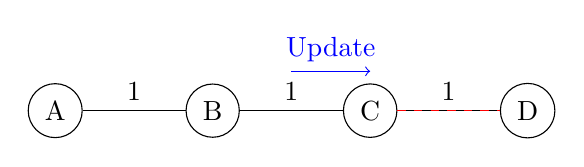
\begin{tikzpicture}[node distance=2cm]
\node[circle,draw] (A) {A};
\node[circle,draw,right of=A] (B) {B};
\node[circle,draw,right of=B] (C) {C};
\node[circle,draw,right of=C] (D) {D};

\draw (A) -- node[above] {1} (B);
\draw (B) -- node[above] {1} (C);
\draw (C) -- node[above] {1} (D);
\draw[red,dashed] (C) -- (D);

\draw[->,blue] (3,0.5) -- node[above] {Update} (4,0.5);
\end{tikzpicture}
\end{figure}

\subsection{Velocità di Convergenza}
La velocità di convergenza, è la velocità con cui un protocollo giunge a convergenza, ossia tutti i router di una rete stanno operando con la stessa visione della rete stessa. 
Problema principale: \textbf{count-to-infinity} (Se un collegamento si interrompe (es. tra B e C), i router potrebbero incrementare all'infinito la distanza (es. A pensa che C sia raggiungibile via B, e B via A)) in reti con loop.
\begin{itemize}
\item Tempo di convergenza \( O(n) \) per reti con \( n \) nodi
\item Aggiornamenti periodici (tipicamente 30 secondi in RIP)
\item Esempio classico:
\begin{verbatim}
A-B-C-D (link C-D si rompe)
B pensa di raggiungere D via A → A pensa di raggiungere D via B
\end{verbatim}
\end{itemize}
\subsection{Poisoned Reverse}
Tecnica per prevenire loop di routing:
\begin{figure}[ht]
\centering
\begin{tikzpicture}[node distance=2cm]
\node[circle,draw] (A) {A};
\node[circle,draw,right of=A] (B) {B};
\node[circle,draw,right of=B] (C) {C};
\draw (A) -- node[above] {1} (B);
\draw (B) -- node[above] {1} (C);
\draw[red,-{Triangle[open]}] (B) to [bend left=45] node[above] {$\infty$} (A);
\end{tikzpicture}
\end{figure}
Logica di funzionamento:
\begin{itemize}
\item Se il percorso ottimo verso \( y \) passa attraverso \( v \)
\item Annuncia a \( v \) costo infinito per \( y \)
\item Previene loop ma riduce l'ottimalità delle rotte
\end{itemize}
\section{Link-State e Dijkstra}
\subsection{Routing Link-State}
Nell'algoritmo di routing Link-State, ogni router
\begin{itemize}
  \item impara il suo ambito locale (linee e nodi adiacenti)
  \item trasmette queste informazioni a tutti gli altri router della rete tramite un \textbf{Link State Packet} (LSP)
  \item memorizza gli LSP tramsessi dagli altri router e costruisce una mappa della rete
  \item calcola in maniera indipendente, le sue tabelle di instradamento applicando alla mappa della rete l'algoritmo di Dijkstra
\end{itemize}
LSP contiene diversi campi
\begin{itemize}
  \item stato di ogni link connesso al router
  \item identità di ogni vicino connesso all'altro estremo del link
  \item costo del link
  \item numero di sequenza per l'LSP (onde evitare informazioni passate)
  \item checksum
  \item lifetime
\end{itemize}
\subsubsection{LSP flooding}
Un LSP viene generato periodicamente, oppure se viene rilevato un cambiamento nella topologia locale (nuovo vicino, cambiamento del costo verso un vicino, persa connettività verso un vicino).
\begin{center}
  \includegraphics[scale=0.7]{./public/lsp.png}
\end{center}
Successivamente alla generazione dell'LSP avviene un operazione di \textbf{flooding}, in cui l'LSP è trasmesso su tutti i link del router, che a loro volta lo trasmetteranno a tutti i loro link. I pacchetti memorizzati nei router formano una mappa completa e aggiornata della rete detta \textbf{Link State Database}
\begin{center}
  \includegraphics[scale=0.7]{./public/linkstatedb.png}
\end{center}
\subsubsection{Gestione LSP}
Alla ricezione di un LSP ci sono 3 casi possibili:
\begin{itemize}
  \item \textbf{LSP nuovo/aggiornato}: il router memorizza il pacchetto e lo ritrasmette in flooding su tutte le linee eccetto quella da cui l'ha spedito
  \item \textbf{LSP con stesso numero di sequenza di quello posseduto}: il router lo ignora e non fa nulla
  \item \textbf{LSP vecchio}: trasmette al mittente il pacchetto più recente
\end{itemize}
\subsubsection{Architettura Link-State}
Un ulteriore componente fondamentale per comporre l'architettura di un router link state, è il \textbf{Forwarding Database}. Ogni router ne produce uno basandosi sul contenuto del Link State Database, e il forwarding database contiente l'insieme delle coppie (path, vicino) per ogni nodo
\begin{center}
  \includegraphics[scale=0.4]{./public/arclinkstate.png}
\end{center}
Ci sono svariati pregi quale la gestione di reti di grandi dimensioni, la rapida convergenza, la minor probabilità di loop, tuttabia è molto complesso da realizzare
\subsection{Algoritmo di Dijkstra}
L'algoritmo di Dijkstra è un metodo per calcolare il percorso più breve da un nodo sorgente a tutti gli altri nodi in un grafo con pesi **non negativi**. È ampiamente utilizzato nei protocolli di routing Link-State, come OSPF.
\subsubsection{Descrizione dell'Algoritmo}
L'algoritmo funziona come segue:
\begin{enumerate}
    \item \textbf{Inizializzazione}:
        \begin{itemize}
            \item Assegna distanza \( 0 \) al nodo sorgente.
            \item Assegna distanza \( \infty \) a tutti gli altri nodi.
            \item Crea una lista di nodi non visitati.
        \end{itemize}
    \item \textbf{Iterazione}:
        \begin{itemize}
            \item Seleziona il nodo non visitato con la distanza minima.
            \item Per ogni vicino del nodo selezionato, calcola la nuova distanza:
                \[
                d(y) = \min\{d(y), d(x) + c(x,y)\}
                \]
                dove:
                \begin{itemize}
                    \item \( d(y) \): distanza corrente verso il nodo \( y \).
                    \item \( d(x) \): distanza dal nodo sorgente al nodo \( x \).
                    \item \( c(x,y) \): costo del collegamento tra \( x \) e \( y \).
                \end{itemize}
            \item Segna il nodo selezionato come visitato.
        \end{itemize}
    \item \textbf{Ripeti} finché tutti i nodi non sono visitati.
\end{enumerate}
\section{Protocollo OSPF (rete)}
Il \textbf{OSPF (Open Shortest Path First)} è un protocollo link-state utilizzato all'interno di sistemi autonomi (IGP). Opera al layer 3 del modello OSI e utilizza l'algoritmo di Dijkstra per calcolare il percorso più breve verso una destinazione. Caratteristiche principali:
\begin{itemize}
    \item Supporta \textbf{VLSM} (Variable Length Subnet Mask) e \textbf{CIDR}
    \item Utilizza multicast (224.0.0.5 e 224.0.0.6) per la comunicazione
    \item Offre autenticazione integrata
    \item Divide le reti in \textbf{aree} per ridurre il traffico di routing
\end{itemize}
\begin{center}
  \includegraphics[scale=0.3]{./public/ospf.jpg}
\end{center}
OSPF prevede 4 tipi di router:
\begin{itemize}
  \item \textbf{Internal router}: tutte le sue interfacce appartengono alla stessa area
  \item \textbf{Area border router}: possiede interfacce in due o più aree distinte
  \item \textbf{Backbone router}: possiede almeno un'interfaccia appartenente all'area 0
  \item \textbf{Autonomous system boundary router}: almeno una delle sue interfacce utilizza un diverso protocollo di routing o appartiene ad un altro AS
\end{itemize}
OSPF è organizzato su una gerarchia ad aree a due livelli, la \textbf{local area} e la \textbf{backbone (area 0)}. Gli Advertisement Link-Sate non lasciano le rispettive aree, dunque i nodi in ogni area hanno una topoliga dettagliata dell'area ma conoscono solo la direzione verso reti in altre aree. Gli Area Border router riassumono distanze a reti nell'area di competenza e le comunicano ad altri router di tipo Area Border. 
\section{Routing gerarchico (rete)}
Nel corso degli anni l'architettura di internet, si è evoluta da un'architettura molto semplice basata su un'unina rete backbone, in cui ogni rete fisica era collegata alla backbone da un core router ad un'architettura più scalabile
\begin{center}
  \includegraphics[scale=0.5]{./public/singlebackbone.png}
\end{center}
Al giorno d'oggi, il routing in internet si basa su reti con \textbf{peer backbone} dando vita al \textbf{routing gerarchico}. 
\begin{center}
  \includegraphics[scale=0.5]{./public/peerbackbone.png}
\end{center}
Internet è strutturato come un'insieme di \textbf{autonomous systems} (AS). Un AS è una collezione limitata di reti amministrate da un'unica autorità con un identificativo AS number di 16 bit. Ogni AS è responsabile del routing all'interno delle sue reti (\textbf{routing interno}) e dello scambio di infromazioni di raggiungibilità con altri AS (\textbf{routing esterno}). Abbiamo dunque due tipi di routing:
\begin{itemize}
  \item Routing interno ad un AS (\textbf{intra-domain routing}), gestito dall'\textbf{Interior Gateway Protocol} (IGP). I messaggi IGP sono scambiati tra router interni all'AS e contengono solo infromazioni sulle reti dell'AS. Questo tipo di routing si basa su protocolli quali:
    \begin{itemize}
      \item RIP (distance vector)
      \item OSPF (link state)
      \item IGRP (Interior Gateway Routing Protocol - Cisco)
    \end{itemize}
  \item Routing esterno tra AS (\textbf{inter-domain routing}), gestito dall'\textbf{Exterior Gateway Protocol} (EGP). I messaggi sono scambiati tra router designati dai rispettivi AS come router di confine (Border Router) e contengono informazioni sulle rotte conosciute dai due AS. Questo tipo di routing si basa su due protocolli:
    \begin{itemize}
      \item EGP (Exterior Gateway Protocol), ormai obsoleto
      \item BGP (Border Gateway Protocol), approccio path vector
    \end{itemize}
\end{itemize}
\subsection{Tipi di AS}
Disitinguiamo gli AS in base ad una serie di caratteristiche. La prima distinzione possibile è quella per dimensione.
\begin{itemize}
  \item \textbf{stub o single homed}: AS con un unico border router
  \item \textbf{multi-homed}: AS con più border router
\end{itemize}
Un ulteriore distinzione è quella riguardante AS transit e non-transit
\begin{itemize}
  \item \textbf{transit AS} (provider): accetta di essere attraversato da traffico diretto ad altri AS
  \item \textbf{non-tranist AS} (grandi corporate): non accetta di essere attraversato da traffico diretto ad altri AS
\end{itemize}
\subsection{Instradamento gerarchico}
L'istradamento gerarchico, organizza la rete in livelli gerarchici per gestire la complessità e migliorare la scalabilità. In BGP gli AS stabiliscono relazioni commerciali che definiscono come il traffico viene scambiato. Ci sono 3 attori principali caratterizzati da diverse relazioni
\begin{enumerate}
  \item \textbf{Customer}: un AS che paga un provider per avere accesso a internet (es: università che paga Telecom). 
    \begin{itemize}
      \item Il provider esporta le routes del customer a tutti gli AS
      \item Il customer esporta le routes del provider ad altri customer del provider
    \end{itemize}
  \item \textbf{Provider}: un AS che vende connettività ad un customer
  \item \textbf{Peer}: due AS che scambiano traffico gratuitamente (peering settlement-free), per reciprocità (Telecom e Vodafone che si connettono direttamente per scambiare traffico dei rispettivi clienti) 
\end{enumerate}
\section{Multicast}
Per \textbf{multicast} si intende un'astrazione in cui l'invio di un pacchetto da un sender a molti receiver avviene con una singola operazione. Si pone di risolvere il problema di invio di pacchetti ad un gruppo specifico di destinatari
\begin{center}
  \includegraphics[scale=0.4]{./public/multicast.png}
\end{center}
Sorge il problema di identificazione dei ricevitori di un datagramma multicast e l'invio del datagramma stesso. Questo avviene tramite \textbf{address indirection}, ossia si utilizza un identificativo unico per il gruppo di ricevitori e una copia del datagramma è inviata utilizzando tale identificativo a tutti i membri del gruppo
\subsection{Indirizzo Multicast IPv4}
Ad ogni gruppo è associato un indirizzo multicast, ossia un indirizzo IP di classe D
\begin{center}
  \includegraphics[scale=0.5]{./public/dclass.png}
\end{center}
\subsection{Multicast ethernet}
Per la trasmissione di datagram IP multicast su reti LAN ethernet, occorre mappare un indirizzo in classe D su di un indirizzo MAC multicast. Questo non è possibile in maniera univoca, dato il range degli indirizzi MAC riservati al multicast (IP multicast 28 bit, MAC multicast 23 bit), dunque 5 bit vengono persi durante il processo di \textbf{aliasing}
\begin{center}
  \includegraphics[scale=0.5]{./public/aliasing.png}
\end{center}
\subsection{Multicast Router}
Il multicast router si occupa dello smistamento dei datagrammi multicast, ciò avviene nel seguente modo
\begin{itemize}
  \item Ogni end system trasmette i datagrammi multicast sfruttando il meccanismo hardware messo a disposizione dalla rete locale su cui si trova
  \item Se un datagramma giunge al multicast router, quest'ultimo si occupa se necessario di instradarlo verso le altre reti
\end{itemize}
\subsection{Protocolli multicast}
Ci sono due protocolli principali per il multicast:
\begin{itemize}
  \item \textbf{Internet Group Managment Protocol (IGMP)}: fornisce ad un host i mezzi per informare il multicast router ad esso più vicino che un'applicazione vuole unirsi ad un determinato gruppo multicast
  \item \textbf{Algoritmi routing}: Coordinano i multicast router all'interno della rete Internet, per permettere l'instradamento dei datagrammi multicast
\end{itemize}
\subsubsection{IGMP}
L'IGMP in tutte le sue versioni (IGMPv1, IGMPv2, IGMPv3) opera tra l'host ed il router ad esso direttamente collegato e serve a gestire in ambito locale le informazioni di membership ai vari gruppi multicast. I messaggi IGMP sono trasmessi in datagrammi IP il cui header ha il campo protocol con valore 2 ed il campo TTL con valore 1. 
\begin{center}
  \includegraphics[scale=0.5]{./public/igmphead.png}
\end{center}
Quando un'applicazione chiede di entrare in un un nuovo gruppo:
\begin{itemize}
  \item l'host in cui gira l'applicazione invia un messaggio IGMP \textbf{membership report}, il messaggio è \textbf{unsolicited} in quanto non generato come risposta ad un messaggio di membership query.
  \item Gli eventuali router multicast presenti nella rete locale dell'host ricevono il messaggio e stabiliscono i meccanismi di routing atti a ricevere i pacchetti indirizzati al gruppo.
\end{itemize}
Dovendo gestire dinamicamente i gruppi, i multicast router, effettuano un'operazione di polling periodica, gli host presenti nelle reti locali collegate rispondono ai messaggi di \textit{membership query} da parte del router con messaggi di \textit{membership report}
\begin{center}
  \includegraphics[scale=0.5]{./public/membership.png}
\end{center}
Un ulteriore protocollo di multicast è il \textbf{source specific multicast}, in cui un host può manifestare l'intenzione a ricevere pacchetti destinati ad un gruppo multicast esclusivamente da uno specifico host sorgente S.
\begin{itemize}
  \item Avviene attraverso un'operazione di \textbf{source specific join} realizzata mediante messaggi IGMPv3 di source specific membership report
\end{itemize}
\begin{center}
  \includegraphics[scale=0.5]{./public/ssm.png}
\end{center}
\subsection{Routing Multicast}
L'obiettivo dell'instradamento multicast è trovare un albero di link che colleghi tutti i router cui sono attaccati gli host che appartengono al gruppo multicast. Ovviamente l'albero può contenere router che non hanno collegati host appartenenti al gruppo multicast.
\begin{center}
  \includegraphics[scale=0.5]{./public/multicastree.png}
\end{center}
Ci sono due approcci possibile alla costruzione dell'albero di percorrenza. 
\begin{itemize}
  \item \textbf{Group Shared Tree}: unico albero condiviso dal gruppo per distribuire il traffico di tutti i mittenti
  \item \textbf{Source-based Tree}: Albero d'instradamento costruito specificamente per ciascun singolo mittente
\end{itemize}
\begin{center}
  \includegraphics[scale=0.5]{./public/multitree.png}
\end{center}
\subsubsection{Group-Shared Tree}
Ci si pone il problema di risolvere lo \textbf{Steiner Tree Problem}, ossia trovare l'albero a costo minimo.
\begin{center}
  \includegraphics[scale=0.3]{./public/groupshared.png}
\end{center}
Si utilizza un approccio centralizzato definendo un nodo centrale come punto di \textbf{rendez-vous/nucleo} (di solito il router con più connessioni adiacenti). 
\begin{itemize}
  \item Tutti i router cui sono collegati host multicast aderiscono al nucleo con messaggi unicast
  \item Il percorso seguito definisce il ramo dell'albero
\end{itemize}
Minimizza la somma dei costi dei link dell'albero multicast
\subsubsection{Source-based Tree}
Si utilizza l'unione dei percorsi minimi dalla sorgente a tutte le destinazioni (\textbf{Least unicast-cost path tree}). 
\begin{center}
  \includegraphics[scale=0.3]{./public/sourcebased.png}
\end{center}
Minimizza il costo dalla sorgente ad ognuna delle destinazioni
\section{MBone (rete)}
La rete \textbf{Multicast BackBone} (MBONE), è una rete virtuale (overlay) composta da "isole" capaci di supportare il forwarding di pacchetti multicast IP collegate mediante link virtuali di tipo punto-punto chiamati \textbf{tunnel}. 
\begin{center}
  \includegraphics[scale=0.5]{./public/backbone.png}
\end{center}
I pacchetti multicast vengono incapsulati prima di essere trasmessi attraverso i tunnel, in modo da apparire all'esame dei router e delle sottoreti intermediarie come normali datagrammi unicast. Un router multicast intenzionato a trasmettere un pacchetto all'altro capo di un tunnel deve aggiungere ad esso un ulteriore header IP in cui sia presente, come indirizzo destinazione, l'indirizzo unicast del router che si trova al capo opposto del tunnel.
\section{IPv6}
La versione IPv6 del protocollo IP, è stata progettata per risolvere alcuni dei prolemi che affligono IPv4. principalmente:
\begin{multicols}{2}
  \begin{itemize}
    \item Indrizzamento e routing
    \item Sicurezza
    \item Configurazione automatica
    \item servizi real-time e supporto alla QoS
    \item elaborazione efficiente dei pacchetti da parte dei router
    \item coesistenza di IPv4 e IPv6
  \end{itemize}
\end{multicols}
La motivazione principale che spinse alla progettazione di IPv6, fu l'esaurimento dello spazio di indirizzi supportati da IPv4.
\subsection{Differenze}
Ci sono 5 differenze principali tra il protocollo IPv6 e IPv4:
\begin{itemize}
  \item \textbf{Espansione capacità di indirizzamento e routing}: la dimensione degli indirizzi passa da 32 bit a 128 bit, viene migliorata la scalabilità del routing multicast grazie all'aggiunta di un campo scope agli indirizzi di classe D e viene definito un nuovo tipo di indirizzo \textbf{anycast address} che si riferisce ad un insieme di interfacce
  \item \textbf{Semplificazione dell'header}: alcuni campi dell'header IPv4 sono eliminati o resi opzionali
  \item \textbf{Supporto per le opzioni migliorato}: alcuni cambiamenti nel modo di codificare le opzioni permettono uno smistamento più efficiente ed una maggior flessibilità, per introdurre nuove funzionalità
  \item \textbf{Supporto della QoS}: introdotta una funzionalità per etichettare i pacchetti appartenenti a flussi di dati particolari per i quali si chiede un trattamento di tipo non-default
  \item \textbf{Autenticazione e salvaguardia della privacy}: definizione di estensioni che forniscono il supporto per autonticazione, integrità dei dati, e la sicurezza.
\end{itemize}
\subsection{Header}
L'header IPv6 consiste di due parti:
\begin{itemize}
  \item \textbf{header principale}
  \item \textbf{extension header} (introdotti per le nuove funzioni)
\end{itemize}
\subsubsection{Header principale}
L'header principale in IPv6 è lungo 40 bit ed è composto nel seguente modo
\begin{multicols}{2}
  \begin{itemize}
    \item \textbf{Version}: 4bit, numero della versione
    \item \textbf{Traffic Class}: 8bit, priorità del pacchetto
    \item \textbf{Flow Label}: 20bit, associa il pacchetto ad un flusso
    \item \textbf{Payload Length}: 16bit, lunghezza del payload (max 64KB)
    \item \textbf{Next Hdr}: 8bit, il tipo di header che segue il principale
    \item \textbf{Hop Limit}: 8bit
    \item \textbf{Source Address}: 128bit, indirizzo mittente
    \item \textbf{Destination Address}: 128bit, indirizzo destinazione
  \end{itemize}
  \includegraphics[scale=0.5]{./public/headeripv6.png}
\end{multicols}
\subsubsection{Extension Header}
Gli extension header sostituiscono il campo options di IPv4, e permettono di specificare opzioni aggiuntive.  Gli extension header se presenti, devono apparire in un ordine preciso
\begin{multicols}{2}
  \begin{itemize}
    \item \textbf{Hop by hop}
    \item \textbf{Routing}
    \item \textbf{Fragment}
    \item \textbf{Authentication}
    \item \textbf{Encrypted security payload}
    \item \textbf{Destination Option}
  \end{itemize}
  \includegraphics[scale=0.3]{./public/extheader.png}
\end{multicols}
\subsection{Indirizzi IPv6}
Un indirizzo IPv6 è formato da 16 byte (128 bit), per la trascrizione degli indirizzi IPv6 si formano otto gruppi di 2 byte ciascuno in cui ciascun gruppo è identificato da cifre esadecimali. Ad esempio
\[\text{2340:0023:AABA:0A01:0055:5054:9ABC:ABB0}\]
Valgono due regole di semplificazione della notazione:
\begin{enumerate}
  \item Una sequenza di zeri all'inizio di un gruppo di 4 cifre può essere omessa
    \[\text{2340:0023:AABA:0A01:0055:5054:9ABC:ABB0}\]
    \[\text{2340:23:AABA:A01:55:5054:9ABC:ABB0}\]
  \item Una sequenza di campi successivi uguali a zero può essere rappresentata con il simbolo "::"
    \[\text{2340:0000:0000:0000:0055:5054:9ABC:ABB0}\]
    \[\text{2340::55:5054:9ABC:ABB0}\]
\end{enumerate}
\begin{itemize}
  \item \textbf{Unicast}: Trasmissione 1 ad 1
  \item \textbf{Multicast}: Trasmissione 1 a molti
  \item \textbf{Anycast}: Trasmissione 1 al più vicino (trasmette al più vicino in un gruppo di molteplici interfacce)
\end{itemize}
Come si nota, non è prevista la trasmissione broadcast
\subsection{Indirizzi IPv6 Unicast}
Gli indirizzi IPv6 unicast si suddividono a loro volta in 3 tipi principali:
\begin{itemize}
  \item \textbf{Global Unicast}: simili agli indirizzi IPv4 pubblici, sono indirizzi pubblici univoci a livello mondiale. Utilizzati per internet o reti pubbliche. Hanno come prefisso \textbf{2000::/3}
    \begin{center}
      \includegraphics[scale=0.5]{./public//globunic.png}
    \end{center}
  \item \textbf{Link Local}: si usano per l'invio di pacchetti nella sottorete locale, hanno come prefisso \textbf{FE80::/10}. Ogni interfaccia di rete su cui è abilitato IPv6 è configurata obbligatoriamente con un indirizzo link-local.
  \item \textbf{Unique Local}: simili agli indirizzi IPv4 privati, hanno come prefisso \textbf{FD00::/8}. Si usano in reti private, non sono inoltrati dai router internet ma possono essere inoltrati da router all'interno di una organizzazione. 
\end{itemize}
Un ulteriore distinzione è quella sul contesto in cui operano gli indirizzi, infatti gli indirizzi IPv6 identificano due ambiti diversi:
\begin{itemize}
  \item \textbf{Link}: comprende tutti i dispositivi in comunicazione diretta tramite una LAN o un collegamento punto-punto
  \item \textbf{Site}: comprende un insieme di link gestiti da un'unica entità (es: campus univeristario)
\end{itemize}
\subsubsection{Indirizzi Link-Local}
Caratterizzati dal prefisso \textbf{FE80::/10}, possono essere utilizzati esclusivamente per comunicare con altri host o router direttamnte raggiungibili tramite un link. Ogni interfaccia di rete che supporti IPv6 deve essere configurata con almeno un IPv6 Link Local
\begin{center}
  \includegraphics[scale=0.5]{./public/linklocal.png}
\end{center}
Il metodo di produzione dell'interface ID varia a seconda del sistema operativo e in generale non vi è garanzia che un indirizzo link local sia globalmente univoco. Con RFC-2373 si definisce un modo per generare un identificativo a 64 bit (EUI-64 extended unique identifier) a partire dal MAC address della scheda di rete.
\begin{itemize}
  \item Si ottiene inserendo al sequenza di 16 bit FF:FE tra i primi ed i secondi 24 bit del MAC address
  \item L'interface ID può essere calcolato a partire da EUI-64 invertendo il settimo bit da sinistra
\end{itemize}
\begin{center}
  \includegraphics[scale=0.5]{./public/EUI.png}
\end{center}
\subsubsection{Indirizzi IPv6 Global Unicast}
Identificati da un prefisso \textbf{2000::/3} identificano un'interfaccia di rete in maniera univoca a livello globale. Sono costituiti da
\begin{itemize}
  \item Un \textbf{subnet ID} da 64 bit, che identifica la sottorete ottenuto aggregando identificatori più piccoli gerarchicamente (Top Level ID, Next Level ID, Site Level ID)
  \item Un \textbf{interface ID} da 64 bit, che identifica l'interfaccia nella sottorete
\end{itemize}
\begin{center}
  \includegraphics[scale=0.5]{./public/globunicast.png}
\end{center}
\subsubsection{Indirizzi IPv6 Multicast}
Iniziano per \textbf{FF::/8} e sono usati come indirizzo destinazione per datagrammi che devono essere inviati a gruppi di device
\begin{center}
  \includegraphics[scale=0.5]{./public/IPv6multicast.png}
\end{center}
\subsection{Assegnazione ad Host}
Esistono diversi modi per attribuire un indirizzo IPv6 ad una interfaccia di host
\begin{itemize}
  \item \textbf{Static Address Configuration}: configurazione statica da parte dell'amministratore
  \item \textbf{Stateless Address-Auto Configuration (SLAAC)}: un indirizzo IPv6 link local è attribuito automaticamente da parte del sistema operativo dell'host
  \item \textbf{Stateful DHCP address assignment}: configurazione dinamica con indirizzo assengato da un server DHCPv6
\end{itemize}
\subsection{ICMPv6}
Si tratta di una variante per IPv6 del protocollo di controllo ICMP. Fornisce funzionalità di controllo, segnalazione errori e diagnostica, ma la vera innovazione risiede nelle funzionalità di \textbf{network discovery}:
\begin{itemize}
  \item \textbf{RS - Router Solicitation}: usati da un host per sollecitare i router raggiungibili direttamente tramite le proprie interfacce a inviare un messaggio di tipo router advertisement
  \item \textbf{RA - Router Advertisement}: usati dai router per manifestare la propria presenza
  \item \textbf{NS - Neighbor Solicitation}: usati da host e router per determinare l'indirizzo link-layer di un vicino o per verificare che un vicino sia ancora raggiungibile tramite indirizzo link-layer in cache
  \item \textbf{NA - Neighbor Advertisement}: inviati in risposta ad un NS, o per annunciare un cambiamento di indirizzo link-layer
  \item \textbf{Redirect}: usati dai router per informare gli hosts dell'esistenza di un router migliore
\end{itemize}
L'address resolution in IPv6 non passa più attraverso il protocollo ARP ma si utilizza ICMPv6
\begin{center}
  \includegraphics[scale=0.5]{./public/ICMPv6.png}
\end{center}
\subsection{Mapping IPv6 - IPv4}
Il mapping degli indirizzi IPv6 su IPv4 avviene attraverso la formazione di indirizzi IPv6 formati da un prefisso di 80 bit "0", 16 bit "1" e il successibo indirizzo IPv4 corrispondente. La notazione è mista, in quanto si usa una notazione esadeciamale per la parte IPv6 e la classica dotted decimal per IPv4, dunque un indirizzo del genere ha la seguente forma
\[\text{0:0:0:0:0:FFFF:w.x.y.z oppure ::FFFF.w.x.y.z}\]
Per la transizione da IPv4 a IPv6 si introduce la nozione di \textbf{tunneling}. I pacchetti IPv6 vengono trasportati come payload all'interno di datagrammi IPv4 tra router IPv4
\begin{center}
  \includegraphics[scale=0.5]{./public/tunnel.png}
\end{center}
\section{Multimedia (trasporto (trasporto))}
Si vuole risolvere il problema di trasferire informazioni multimediali da una sorgente ad uno o più ricevitori attraverso una rete. Il processo è teoreticamente semplice e composto da 3 step:
\begin{itemize}
  \item il \textbf{trasmettitore} si occupa di effettuare una compressione secondo una opportuna tecnica (MPEG, MJPEG, MP3) per ridurre la quantità di informazioni da trasferire
  \item la \textbf{rete} trasmette l'informazione in pacchetti
  \item il \textbf{ricevitore} recupera l'informazione originaria dalla sequenza di pacchetti ricevuti mediante un'operazione inversa a quella di compressione e una successiva trasformazione in forma sonora o di video
\end{itemize}
C'è una necessaria differenza tra informazioni \textbf{live} e \textbf{pre-registrate}
\begin{itemize}
  \item nelle informazioni live, l'informazione è prodotta e compressa mediante un apposito sistemaprima della trasmissione
  \item nel caso di informazioni pre-registrate, l'informazion è già registrata in formato compresso e memorizzata su memoria di massa prima di effettuare la trasmissione
\end{itemize}
\subsection{Live/Pre-registrate}
\subsubsection{Pre-registrate}
Esistono due modalità di fruizione
\begin{itemize}
  \item \textbf{File-Transfer}: Avviene il trasferimento dell'intero file da sorgente a ricevitore e successivamente la riproduzione.
  \begin{itemize}
    \item La riproduzione può iniziare solo al termine della trasmissione e necessita di capacità di memorizzazione adeguate
  \end{itemize}
\item \textbf{riproduzione progressiva}: La riproduzione avviene durante il trasferimento
  \begin{itemize}
    \item Il ricevitore memorizza l'informazione in un buffer (\textbf{playout buffer}) che viene progressivamente alimentato e svuotato
  \end{itemize}
\end{itemize}
\subsubsection{Live}
Nel caso di informazioni live, la sorgente produce un flusso continuo di informazioni. Questo flusso di informazioni è spezzato in \textbf{pacchetti} che sono trasmessi individualmente sulla rete in un processo definito \textbf{streaming}. Lo streaming è molto sensiile alla QoS:
\begin{itemize}
  \item il ricevitore riesce a recuperare la continuità del flusso di pacchetti se tutti i pacchetti arrivano a destinazione con la stessa tempificazione relativa
  \item La rete può alterare la continuità temporale facendo occasionalmente perdere pacchetti o consegnando pacchetti con tempificazione diversa da quella in cui sono stati trasmessi (\textbf{jitter})
\end{itemize}
Per arginare il problema rispetto alla perdita occasionale di pacchetti, cis si difende mediante tecniche di compressione robuste, per le quali l'informazione audio/video non è sensibilmente degradata quando occasionalmente si perde un pacchetto. Per limitare il problema del jitter, si adotta una strategia di bufferizzazione
\section{RTP/RTCP (applicativo/trasporto)}
Il trasferimento di informazioni pre-registrate avviene mediante file transfer realizzato attraverso HTTP/TCP. Per la trasmissione in streaming vengono invece adottate 2 tecniche, HTTP/TCP o un protocollo ad-hoc RTP su UDP.
\subsection{RTP}
Il \textbf{Real-Time Transport Protocol (RTP)} offre un servizio a livello di trasporto specificamente progettato per i requisiti di flussi multimediali. I pacchetti RTP sono incapsulati in datagrammi UDP
\begin{itemize}
  \item è concepito per essere implementato a livello applicativo e non come uno strato aggiuntivo dello stack protocollare
  \item offre funzinalità minimali richieste dalla trasmissione di flussi continui tipici delle applicazioni multimediali
  \item è neutrale rispetto alla codifica utilizzata
\end{itemize}
Risolve il problema dello jitter. RTP fornisce informazioni di tempificazione (\textbf{timestamps}), Esistono due tipi di sincronizzazione
\begin{itemize}
  \item \textbf{Sincronizzazione Intra-Media}: ricostruzione corretta della tempificazione della sequenza di pacchetti ricevuti
  \item \textbf{Sincronizzazione Inter-Media}: con lo scopo di mantenere sincronizzati flussi multimediali trasmessi separatamente (es. audio e video e lip-sync)
\end{itemize}
Supporta sia la trasmissione unicast che multicast e i suoi meccanismi sono scalabili rispetto al numero di appartenenti al multicast.
\subsection{Struttura}
Un pacchetto RTP è trasmesso in un datagramma UDP
\begin{center}
  \includegraphics[scale=0.5]{./public/rtp.png}
\end{center}
L'header UDP contiene i numeri di porto sorgente e destinazione, RTP usa numeri di porto destinazione pari per la trasmissione dei flussi di dati, lasciando il numero dispari successivo al protocollo RTCP per trasmettere informazioni di controllo relative a quel flusso.
\subsubsection{Header RTP}
L'header RTP è formato nel seguente modo
\begin{center}
  \includegraphics[scale=0.5]{./public/headerrtp.png}
\end{center}
\begin{itemize}
  \item \textbf{Payload Type}: 7 bit, specifica la codifica utilizzata per i dati
  \item \textbf{Sequence Number}: 16 bit, serve ad identificare le perdite di pacchetti
  \item \textbf{Timestamps}: 32 bit, specifica il tempo di campionamento del primo byte del payload
  \item \textbf{Synchronization Source Identifier (SSRC)}: 32 bit, identifica la sorgente del flusso, ed è scelto casualmente dalla sorgente stessa
  \item \textbf{Contributing Source Identifier (CSRC)}: sequenza di n campi da 32 bit (n compresa tra 0 e 15), ciascuno dei quali identifica la sorgente originaria in un flusso prodotto dalla "fusione" di flussi diversi mediante un mixer software (es. in una videoconferenza SSRC identifica il mixer, CSRC indica lo speaker corrente)
\end{itemize}
\subsection{Sessione RTP}
Una associazione tra un gruppo di entità che comunicano mediante RTP è definita \textbf{Sessione}. Sessioni differenti vengono distinte da un recivitore mediante il port number di livello trasporto (UDP)
\subsection{RTCP}
Si tratta del protocollo utilizzato congiuntamente ad RTP per la trasmissione di informazioni di controllo. I pacchetti RTCP vengono inviati con una certa periodicità e trasportano informazioni di varia natura:
\begin{itemize}
  \item feedback sulla qualità della ricezione dei dati
  \item identificazione dei partecipanti ad una sessione RTP
\end{itemize}
Il protocollo RTCP definisce cinque tipi diversi di messaggi:
\begin{itemize}
  \item \textbf{Source Report - SR}
  \item \textbf{Receiver Report - RR}
  \item \textbf{Source Description - SD}
  \item \textbf{BYE}
  \item \textbf{APP}
\end{itemize}
I messaggi di tipo report contengono statistiche sul numero di pacchetti inviati, ricevuti... I messaggi di tipo description contengono informazioni sulla sorgente del flusso, BYE serve a notificare l'uscita da una sessione, APP permette di definire la sua funzione all'interno dell'applicazione
\section{Trasmissione affidabile (trasporto)}
Se il livello rete è inaffidabile, nella comunicazione end-to-end si potrebbero verificare sitauzioni quali perdita di pacchetti, presenza di errori, ordine dei pacchetti non garantito ecc... È il livello di trasporto che si occupa di mitigare questi problemi.
\subsection{Soluzioni}
Nel caso in cui ci siano errori in trasmissione da parte della rete, il ricevente deve effettuare 2 step:
\begin{enumerate}
  \item Rilevamento degli errori
  \item Correzione degli errori o notifica al mittente richiesta di ritrasmissione
\end{enumerate}
La prima soluzione introduce complicazioni, la seconda introduce possibili duplicazioni sulla rete che il ricevente non è in grado di interpretare.
\begin{center}
  \includegraphics[scale=0.5]{./public/acknak.png}
\end{center}
Per risolvere il problema dei duplicati, occorre inserire nell'header del segmento da inviare un \textbf{numero di sequenza}.
\subsection{Stop and Wait}
Si definiscono protocolli \textbf{Stop \& Wait} quei protocolli che inviano un messaggio e attendono un riscontro prima di ritrasmettere un nuovo messaggio. Per questo tipo di protocolli è sufficiente un numero di sequenza ad un bit per realizzare una trasmissione affidabile.
\begin{center}
  \includegraphics[scale=0.5]{./public/stopwait.png}
\end{center}
È possibile realizzare un protocollo del genere anche senza NAK, ma facendo in modo che il destinatario invii un ACK per l'ultimo pacchetto ricevuto correttamente che includa il numero di sequenza. Tuttavia in questo modo stiamo gestendo solo il caso dei duplicati, per gestire la perdita di pacchetti è necessario introdurre come paramtro un \textbf{timeout}, allo scadere del quale, se non è stato ricevuto il segnale di ACK dal destinatario, il pacchetto viene reinviato.
\begin{center}
  \includegraphics[scale=0.5]{./public/timeout.png}
\end{center}
\subsection{Pipelining}
In alternativa allo stop and wait, si può utilizzare la tecnica del \textbf{Pipelining}, in cui il mittente invia pacchetti prima di ricevere il riscontro dei precenti, e successivamente riceve i segnali di ack dei vari pacchetti da parte del destinatario. Ne esistono due versioni: \textbf{go-Back-N} e \textbf{Selective Repeat}
\begin{center}
  \includegraphics[scale=0.5]{./public/pipelining.png}
\end{center}
\subsubsection{Go Back-N}
Nel go back-n, vengono inseriti nell'header del segmento k bit per il numero di sequenza, successivamente, si stabilisce una finestra di max N pacchetti senza riscontro.
\begin{center}
  \includegraphics[scale=0.5]{./public/gobackn.png}
\end{center}
Gli ack ricevuti sono numerati e cumulativi, ciò implica che ricevere ACK(n) vuol dire che tutti i pacchetti precedenti all'ennesimo sono stati ricevuti correttamente. 
\begin{center}
  \includegraphics[scale=0.5]{./public/gobacknact.png}
\end{center}
\subsubsection{Ripetizione selettiva}
Il riceventi invia riscontri specifici per tutti i pacchetti ricevuti correttamente e il mittente ritrasmette soltanto i pacchetti per i quali non ha ricevuto un ACK. 
\begin{center}
  \includegraphics[scale=0.5]{./public/selettiverepeat.png}
\end{center}
\section{TCP}
Il \textbf{Trasmission Control Protocol (TCP)} è un protocollo di trasporto connection oriented che consente la trasmissione bidirezionale affidabile di un flusso di byte tra due endpoint. 
\subsection{Struttura}
La struttura di un segmento TCP è la seguente
\begin{center}
  \includegraphics[scale=0.5]{./public/tcpstruct.png}
\end{center}
\begin{itemize}
    \item \textbf{N. Porta Sorgente/Destinazione}
    \item \textbf{Lunghezza Header HLEN}: 4 bit, assume valori tra 5 e 15 (da 20byte a 60byte)
    \item \textbf{Numero di sequenza}: idenifica nello stream di byte la posizione dei dati nel segmento
    \item \textbf{Numero di riscontro}: contine il numero sequenziale del byte successivo a quello ricevuto correttamente dalla destinazione (valido solo negli ACK=1)
    \item \textbf{Flag}: per identificare il tipo di informazione contenuta nel segmento
    \item \textbf{Finestra di ricezione}: numero intero di 16 bit che specifica la dimensione del buffer che il TCP ha a disposizione per immagazzinare i dati in arrivo
    \item \textbf{Puntatore ai dati urgenti}: se falg URG=1, contiene il puntatore alla posizione nello stream dei dati non urgenti (ultimo byte dati urgenti)
    \item \textbf{Checksum}: Campo di 16 bit contente un valore intero per verificare l'integrità del segmento
\end{itemize}
Alcuni segmenti speciali sono i segmenti con flag ACK, definiti \textbf{segmenti di riscontro}. Un segmento inviato da B ad A può contenere o meno dati relativi allo stream, e può contenere o meno dati di riscontro, se li contiene entrambi si definisce (\textbf{piggy-backing}).
\subsubsection{Opzioni header TCP}
Le opzioni sono di lunghezza variabile, ma la lunghezza totale dell'header TCP deve essere multipla di 4 byte. Ci sono due formati per le opzioni
\begin{center}
  \includegraphics[scale=0.5]{./public/opzioniheader.png}
\end{center}
Ci sono vari valori che può assumere il campo options dell'header TCP:
\begin{itemize}
  \item \textbf{MSS}: durante la fase di connessione, ciascun end-point annuncia la massima dimensione di payload (MSS - Maximum Segment Size) che desidera accettre 
  \item \textbf{Window Scale}: Per negoziare un fattore di scala per la finestra
  \item \textbf{Selective Repeat}: Nel caso in cui un segmento corrotto sia stato seguito da segmenti corretti, introdice i NAK per permettere al receiver di richiedere la ritrasmissione di quello specifico segmento
  \item \textbf{Timestamps}: utilizza i timestamps per aiutare i due endpoint a determinare il Round Trip Time
  \item \textbf{NOP}: No-Operations, separa opzioni diverse quando non llineate su miltipli di lunghezza di quattro byte
  \item \textbf{EOL}: End of Options List, indica la fine delle opzioni necessario se la fine delle opzioni non coincide con la fine dell'header TCP
\end{itemize}
\subsection{Affidabilità}
Per mantenere standard di affidabilità, TCP si basa su 
\begin{itemize}
  \item \textbf{Riscontro e trasmissione}: consiste nella ritrasmissione di un segmento se non è giunta conferma entro un tempo massimo (time out)
  \item \textbf{Time-Out}: Al momento della trasmissione di un segmento, il TCP attiva un timer
\end{itemize}
TCP vede i dati come un flusso di byte non strutturati ma ordinate in base a \textbf{numeri di sequenza progressivi}. Se consideriamo un flusso di 500.000 byte, con MSS 1000 byte, ci saranno 500 segmenti con numeri di sequenza 1000, 2000, ... All'inverso il \textbf{numero di riscontro} contiene il numero di sequenza del byte successivo a quello ricevuto correttamente dalla destinazione
\begin{center}
  \includegraphics[scale=0.4]{./public/ackseq.png}
\end{center}
Per quanto riguarda il secondo meccanismo, ossia il meccanismo di Time-Out, il problema è a che valore impostare il timeout? Il problema sta nello stimare RTT correttamente. La stima di RTT avviene tramite media esponenziale pesata dei campioni e la stima della deviazione di RTT.
\begin{center}
  \includegraphics[scale=0.5]{./public/stimartt.png}
\end{center}
il valore del timeout è dato da
\[\text{Timeout}=\text{EsitamatedRTT}+4*\text{DevRTT}\]
\subsection{Connection Establishment}
La procedura per stabilire una connessione è detta \textbf{Three-way-handshake}. Ed è sintetizzata dal seguente schema
\begin{center}
  \includegraphics[scale=0.5]{./public/threewayhand.png}
\end{center}
Nella fase three-way handshake, i due endpoint allocano i buffer per i dati e concordano sui valori iniziali dei numeri di sequenza da utilizzare per gli stream dati in entrambi i versi:
\begin{enumerate}
  \item client invia il segmento di controllo TCP SYN al server
  \item cerver riceve SYN e risponde con segmento di controllo SYN/ACK
  \item client riceve SYN/ACK e invia ACK al server
\end{enumerate}
In seguito a questo scambio, viene instaurata la connessione, in cui le due parti apprendono il valore iniziale di Recv Window e utilizzano le opzioni TCP per determinare il valore di MSS, RTT ecc... Per quanto riguarda la connection termination, si utilizza la procedura \textbf{four-way-handshake} in cui la parte che manifesta la volontà di chiudere la trasmissione si chiama \textbf{active closer} e l'altra parte \textbf{passive closer}, la procedura segue questi step
\begin{enumerate}
  \item l'active closer invia un segmento FIN
  \item il passive closer invia un segmento ACK/FIN
  \item l'active closer attende in uno stato TIME\_WAIT tipicamente di 120s
  \item l'active closer invia una ACK di chiusura al passive closer e al termine della TIME\_WAIT chiude
\end{enumerate}
\begin{center}
  \includegraphics[scale=0.5]{./public/4wayhand.png}
\end{center}
\subsection{Schema riassuntivo ACK}
Di seguito uno schema che riassume gli ACK da cosa vengono generati e le azioni conseguenti
\begin{center}
  \includegraphics[scale=0.5]{./public/ackschema.png}
\end{center}
\subsection{Flow Control}
Il controllo di flusso è necessario per risolvere i problemi di sincronizzazione tra invio e lettura di due endpoint. Ci possono essere due bottleneck
\begin{itemize}
  \item \textbf{Receiver Window}: dimensione del buffer di ricezione troppo piccola
  \item \textbf{Congestion Window}: congestione all'interno della rete
\end{itemize}
\begin{center}
  \includegraphics[scale=0.5]{./public/flowcontrol.png}
\end{center}
Il \textbf{receiver buffer} è strutturato così
\begin{center}
  \includegraphics[scale=0.5]{./public/recvbuff.png}
\end{center}
Il mittente non dovrà sovraccaricare il recevente inviando dati nel \textbf{receiver buffer} ad una velocità troppo elevata ciò avviente nel seguente modo
\begin{itemize}
  \item \textbf{ricevente}: comunica dinamicamente al mittente la dimensione corrente del buffer nel campo \textbf{RcvWindow}
    \[\text{RcvWindow}=\text{RcvBuffer} - [\text{LastByteRcvd}-\text{LastByteRead}]\]
  \item \textbf{mittente}: conserva i dati già trasmessi ma non riscontrati e limita tale quantità all'ultima RcvWindow ricevuta
\end{itemize}
\subsection{Congestion Control}
In caso di un numero elevato di sorgenti di traffico, sorgenti che inviano troppi dati o traffico inviato a frequenza troppo elevata, la rete può andare in contro a un sovraccarico. Questa situazione si definisce come \textbf{congestione della rete}. Ci sono due approcci per mitigare questo problema
\begin{itemize}
  \item \textbf{Approccio end-to-end}: non prevede segnalazione esplicita dalla rete, ma gli end-systems a partire dall'osservazione dei ritardi e perdite di pacchetti deducono uno stato di congestione (approccio utilizzato in TCP)
  \item \textbf{Approccio a segnalazione della rete}: i router forniscono informazioni circa lo stato della rete agli end-system
\end{itemize}
\begin{center}
  \includegraphics[scale=0.5]{./public/congcontrol.png}
\end{center}
\subsubsection{TCP congestion control}
Il protocollo TCP implementa un controllo end-to-end a frequenza di trasmissione variabile
\begin{center}
  \includegraphics[scale=0.5]{./public/congwin.png}
\end{center}
La frequenza di trasmissione dipende dalla \textbf{CongWin}, ossia la finestra di congestione. Il risultato considerando il controllo di flusso e controllo di congestione è
\[\text{LastByteSent - LastByteAcked} \leq \text{min\{RcvWindow,CongWin\}}\]
Si procede per tentativi per stabilire quanti si può trasmettere, con l'obiettivo di trasmettere alla massima velocità possibile senza perdite. L'approccio utilizzato è 
\begin{itemize}
  \item Incrementare CongWin finchè non si verifica la perdita di un segmento 
  \item In seguito alla perdita di un segmento si decrementa CongWin e si ricomincia da capo
\end{itemize}
Le fasi di controllo della gestione si definiscono
\begin{itemize}
  \item \textbf{Slow Start}: si incrementa esponenzialmente la dimensione della CongWin ad ogni RTT fino al verificarsi di un evento di perdita (timeout, tre ACK duplicati consecutivi) e si ritrona a CongWin = 1 MSS
  \item \textbf{Congestion Avoidance}: una volta raggiunta la soglia si entra in questa fase in cui ci si avvicina con cautela al valore della banda disponibile tra le due estremità della connessione incrementanto CongWin di
    \[\text{CongWin = CongWin + MSS (MSS/CongWin)}\]
    Al sopraggiungere della congestione, se
    \begin{itemize}
      \item scade un timeout: slow start
      \item tre ACK duplicati consecutivi (TCP Tahoe): slow start
      \item tre ACK duplicati consecutivi (TCP Reno): fast recovery
    \end{itemize}
\end{itemize}
Il concetto di \textbf{Fast Recovery} è implementato in TCP Reno ed elimina la fase di slow start dopo la ricezione di 3 ACK duplicati. Tale evento indica che nonostante sia perso un pacchetto, almeno 3 segmenti successivi sono stati ricevuti dal destinatario, dunque la rete è in grado di consegnare una certa quantità di dati. La CongWin viene dunque aumentata come
\[\text{Threshold = CongWin/2}, \text{     CongWin = Threshold + 3MSS}\]
\begin{center}
  \includegraphics[scale=0.5]{./public/reno.png}
\end{center}
\section{Ethernet (data link)}
Iniziamo sancendo in modo netto la differenza tra indirizzi IP a 32 bit e indirizzi LAN
\begin{itemize}
  \item \textbf{Indirizzi IP}: sfruttati da parte del layer 3 rete per permettere la corretta consegna del pacchetto ad un destinatario collegato alla rete
  \item \textbf{Indirizzi LAN (o MAC o fisici)}: isati per permettere la trasmissione di un frame da una scheda di rete ad un'altra con cui sussiste un collegamento diretto (stessa rete fisica). Si tratta di indirizzi MAC di 48 bit per la maggior parte delle LAN cablati nella ROM delle schede di rete 
\end{itemize}
\subsection{Indirizzi LAN}
La distribuzione degli indirizzi MAC è gestita dall'IEEE e i costruttori di schede di rete detengono una porzione degli indirizzi MAC per garantirne l'univocità. Gli indirizzi MAC si compongono di 2 parti grandi 3 byte ciascuna:
\begin{center}
  \includegraphics[scale=0.5]{./public/macaddr.png}
\end{center}
I tre byte più significativi indicano il lotto di indirizzi acquistato dall'IEEE e si definisce \textbf{Organization Unique Identifier (OUI)}. Gli ultimi 3 byte vengono invece assegnati in base a numerazione progressiva dal costruttore. Gli indirizzi MAC si dividono in 3 tipi
\begin{itemize}
  \item \textbf{single}: di una singola stazione
  \item \textbf{multicast}: di un gruppo di stazioni
  \item \textbf{broadcast}: di tutte le stazioni (ff-ff-ff-ff-ff-ff)
\end{itemize}
Ogni scheda di rete, quando riceve un pacchetto lo passa ai livelli superiori nei seguenti casi
\begin{itemize}
  \item broadcast: sempre
  \item multicast: se ne è stata abilitata la ricezione via software
  \item single: se il DSAP è uguale a quello hardware della scheda o a quello caricato da software in un apposito buffer
\end{itemize}
\subsection{Ethernet}
L'ethernet è la tecnologia dominante per la LAN dato il costo ridotto, vediamo come opera al livello 2. L'interfaccia di rete del mittente incapsula i datagrammi IP in \textbf{frame ethernet} strutturati nel seguente modo
\begin{center}
  \includegraphics[scale=0.5]{./public/frameth.png}
\end{center}
\begin{itemize}
  \item \textbf{Preambolo (8 byte)}: utilizzato per sincronizzare i clock di mittente e destinatario
  \item \textbf{Indirizzi (6 byte)}: la frame è ricevuta da tutti gli adattatori di rete presenti sulla LAN e scartata se l'indirizzo non coincide con quello della scheda stessa
  \item \textbf{Type (2 byte)}: indica il protocollo di rete sovrastante, principalmente IP
  \item \textbf{CRC (4 byte)}: per il controllo effettuato alla destinazione
\end{itemize}
Ogni frame viene trasmessa dopo un \textbf{inter frame gap} corrispondente al tempo di trasmissione di 12 Byte.
La dimensione minima di una frame Ethernet = 64 byte, 14 Byte di header + un minimo di 46 Byte per la PDU e 4 Byte per la CRC. Tuttavia in trasmissione considerando il Preamble di 8 byte e la interframe gap di 12 si ha una dimensione minima di 84 byte. Con dimensione del PDU massima si ha una dimensione massima di 1538 Byte.
\subsubsection{CSMA/CD}
Il \textbf{Carrier Sense Multiple Access w Collision Detection (CSMA/CD)} è un protocollo di accesso multiplo utilizzato nelle reti Ethernet per gestire la trasmissione dei dati su un mezzo condiviso. Lo scopo principale è permetteree a più dispositivi di condividere lo stesso canale di comunicazione evitando collisioni o gestendole se si verificano. Opera su 3 attori principali
\begin{itemize}
  \item \textbf{Jam Signal}: consente alle altri stazioni di accorgersi dell'avvenuta collisione (48 bit)
  \item \textbf{Exponential Backoff}: un algoritmo per adattare i successivi tentativi di ri-trasmissione al carico corrente della rete
  \item \textbf{Segnale}: segnale in codifica Manchester
\end{itemize}
L'algoritmo di backoff fa si che dopo $n$ collisioni il dispositivo attende un tempo casuale compreso tra 0 e $2 -1$ "slot time". Lo slot time è il tempo minimo per trasmettere 512 bit, dopo 10 collisioni consecutive l'intervallo si stabilizza a un limite massimo di 1023 slot
\begin{center}
  \includegraphics[scale=0.5]{./public/csma.png}
\end{center}
\subsection{Standard Ethernet Storici e Moderni}
Gli standard Ethernet si differenziano per velocità, tipo di cavo e topologia. Di seguito i principali:
\begin{itemize}
    \item \textbf{10BASE5} ("Thick Ethernet"):
    \begin{itemize}
        \item Cavo coassiale spesso (10 mm), \textbf{10 Mbps}, lunghezza massima \textbf{500 m}.
        \item Topologia a bus, con connessioni a "vampiro" (transceiver agganciati al cavo).
        \item Obsoleto, utilizzato negli anni '80.
    \end{itemize}
    \item \textbf{10BASE2} ("Thin Ethernet"):
    \begin{itemize}
        \item Cavo coassiale sottile (5 mm), \textbf{10 Mbps}, lunghezza massima \textbf{185 m}.
        \item Connettori BNC a baionetta, topologia a bus senza hub.
        \item Più economico del 10BASE5, ma sostituito dal twisted pair.
    \end{itemize}
    \item \textbf{10BASE-T} (IEEE 802.3i):
    \begin{itemize}
        \item Cavo UTP Cat3, \textbf{10 Mbps}, lunghezza massima \textbf{100 m}.
        \item Topologia a stella con hub, connettori RJ-45.
        \item Rivoluzionario per la semplicità di installazione (anni '90).
    \end{itemize}
    \item \textbf{100BASE-TX} ("Fast Ethernet"):
    \begin{itemize}
        \item Cavo UTP Cat5 o superiore, \textbf{100 Mbps}, stessa lunghezza (100 m).
        \item Utilizza 2 coppie twisted pair, compatibile con il formato frame 10BASE-T.
        \item Dominante negli anni 2000, ancora utilizzato per dispositivi legacy.
    \end{itemize}
\end{itemize}

\subsection{Differenze tra Cavi UTP}
I cavi UTP (Unshielded Twisted Pair) sono classificati in categorie in base a velocità e frequenza:

\begin{table}[h]
\centering
\begin{tabular}{|l|c|c|c|}
\hline
\textbf{Categoria} & \textbf{Banda} & \textbf{Max Velocità} & \textbf{Applicazioni} \\
\hline
Cat3 & 16 MHz & 10 Mbps & 10BASE-T (obsoleto) \\
Cat5 & 100 MHz & 100 Mbps & 100BASE-TX, Fast Ethernet \\
Cat5e & 100 MHz & 1 Gbps & Gigabit Ethernet (base) \\
Cat6 & 250 MHz & 10 Gbps & Gigabit/10G (fino a 55 m) \\
Cat6a & 500 MHz & 10 Gbps & 10 Gigabit Ethernet (100 m) \\
\hline
\end{tabular}
\end{table}
\begin{itemize}
    \item \textbf{Shielding}: I cavi UTP non hanno schermatura (a differenza di STP o FTP), ma usano torsioni delle coppie per ridurre le interferenze.
    \item \textbf{Compatibilità}: Cavi di categoria superiore sono retrocompatibili (es. Cat6 può sostituire Cat5).
    \item \textbf{Distanza}: Tutte le categorie supportano fino a 100 m, tranne Cat6 per 10 Gbps (limitato a 55 m).
\end{itemize}
\section{Dispositivi LAN (data link)}
\subsection{Hub}
Gli hub sono dispositivi di livello fisico che fungono sostanzialmente da ripetitori di bit.
\begin{itemize}
  \item riproducono i bit in ingresso ad un'interfaccia su tutte le altre interfacce
\end{itemize}
\begin{center}
  \includegraphics[scale=0.5]{./public/hub.png}
\end{center}
Gli hub sono organizzati in una gerarchia \textbf{multi-livello} con un backbone hub al livello più alto. Ogni LAN collegata si dice \textbf{segmento di LAN}
\begin{center}
  \includegraphics[scale=0.5]{./public/hubge.png}
\end{center}
Interconnessione tramite hub ha sia pro:
\begin{itemize}
  \item L'organizzazione multi livello grantisce una parziale tolleranza ai guasti
  \item Si estende la massima distanza tra i nodi
\end{itemize}
che contro:
\begin{itemize}
  \item Gli hub non isolano i domini di collisione, le stazioni di un segmento possono subire una collisione per una trasmissione simultanea da parte di una stazione presente su un qualunque altro segmento
  \item La creazione di un singolo dominio di collisione non comporta aumento del throughput massimo
  \item La realizzazione di un unica LAN impone un limite al numero massimo di stazioni che è possibile collegare, nonchè all'estensione geografica che è possibile raggiungere
\end{itemize}
\subsection{Bridge}
I bridge sono dispositivi che permettono il collegamento di due o più LAN tra loro in maniera più efficiente degli Hub. I bridge filtrano i pacchetti, ossia se al destinazione è sullo stesso segmento LAN del mittente, il bridge non compie nessuna azione, se è su un segmento di LAN differente, inoltra il frame sul segmento LAN appropriato. Per scoprire a quali interfacce sono collegati gli host, i bridge eseguono un algoritmo di \textbf{autoapprendimento}. 
\begin{itemize}
  \item Salvano informazioni in tabelle dette \textbf{filtering tables}
  \item Quando una frame è ricevuta il bridge salva il segmento di LAN di provenienza in una filtering table
  \item Una entry nella filtering table è composta da MAC Address, Bridge Port, Time Stamp
\end{itemize}
\begin{center}
  \includegraphics[scale=0.5]{./public/filteringtable.png}
\end{center}
I vantaggi dei bridge sono:
\begin{itemize}
  \item Isolano i domini di collisione, determianndo un aumento complessivo del throughput massimo
  \item Non introducono limitazioni sul numero massimo delle stazioni
  \item Possono collegare differenti tecnologie
  \item Sono trasparenti, ossia nn richiedono alcuna modifica negli adattatori del computer nè configurazione da parte di un admin
\end{itemize}
\subsection{Switch}
Gli switch ethernet sono dispositivi il cui comportmento è simile a quello di un bridge. Sono dispositivi con diverse porte di rete e fungono da centro stella del cablaggio in modo simile ad un hub, tuttavia la superiorità di uno switch rispetto a bridge e hub è dovuta al fatto che inoltra le frame solo verso la porta del destinatario grazie ad un'azione di filtraggio
\begin{center}
  \includegraphics[scale=0.5]{./public/switch.png}
\end{center}
Il principale vantaggio di questo tipo di filtraggio, è la totale assenza di collisioni tra porte distinte. Sono molto rapidi ad operare grazie al \textbf{Cut-through switching}, ossia l'inoltro delle frame verso la porta di uscita corrispondente prima che il frame sia stato ricevuto completamente (basta ricevere l'header del frame per stabilire la porta di uscita)
\section{VLAN (data link)}
Una \textbf{Virtual Local Area Network (VLAN)} è una tecnologia di rete che permette di suddividere una rete fisica in più reti logiche indipendenti. Funziona al livello 2 del modello OSI e offre vantaggi significativi in termini di sicurezza, gestione del traffico e flessibilità organizzativa. 
\begin{center}
  \includegraphics[scale=0.5]{./public/valn.png}
\end{center}
È costituita da switch ehernet che supportano la VLAN e attraverso questi ultimi è possibile raggruppare gruppi di porte tra le quali è possibile una comunicazione diretta e l'inoltro di traffico broadcast. La comununicazione tra VLAN diverse rimane tuttavia possibile solo attraverso una funzione L3 di routing
\subsection{Funzionamento}
Come detto in precedenza, una VLAN permette l'interconnessione di switch Ethernet in LAN virtuali, tipicamente coincidenti con una sottorete IP. Vediamo la differenza tra una rete con VLAN e senza
\begin{itemize}
  \item \textbf{Senza VLAN}: ogni gruppo ha una sottorete IP differente e uno switch ethernet differente
    \begin{center}
      \includegraphics[scale=0.5]{./public/wwlan.png}
    \end{center}
  \item \textbf{Con VLAN}: lo swith è configurato con le porte appropriate per ogni VLAN. Ogni gruppo ha ancora una sottorete IP differente, ma sono tutte collegate allo stesso switch
    \begin{center}
      \includegraphics[scale=0.5]{./public/wvlan.png}
    \end{center}
\end{itemize}
Esistono 3 tipi principali di VLAN:
\begin{itemize}
  \item \textbf{Port-based}: è il metodo più comune, le porte sono assegnate individualmente, in gruppi, in righe o attraverso 2 o più switch. Spesso sono implementate con DHCP per assegnare indirizzi IP agli host del network
  \item \textbf{MAC address}: meno comuni, ogni indirizzo MAC deve essere assegnato allo switch e configurato individualmente. Difficili da gestire
  \item \textbf{Protocol Based}: Si configurano come le MAC address ma utilizzano l'indirizzo IP degli host. Non più comuni a causa dei DHCP
\end{itemize}
La gestione dei messaggi in broadcast, è decisamente più ottimale attraverso l'uso delle VLAN. 
\begin{itemize}
  \item \textbf{Senza VLAN}: ogni host a prescindere della sottorete connesso allo switch riceve il messaggio in broadcast (ad esempio ARP message)
  \item \textbf{Con VLAN}: solo gli host all'interno della rete virtuale ricevono il messaggio in broadcast
\end{itemize}
L'assegnazione degli host, va fatta sulle porte dello switch, e per far si che un host sia parte della VLAN, deve ricevere un indirizzo IP che appartiene alla sottorete appropriate (VLAN = Subnet). L'assegnazione di un host alla corretta VLAN è un processo di due step
\begin{itemize}
  \item Connettere l'host alla porta corretta sullo switch
  \item Assegnare all'host l'indirizzo IP corretto a seconda della appartenenza alla VLAN
\end{itemize}
\begin{center}
  \includegraphics[scale=0.5]{./public/vlanass.png}
\end{center}
La configurazione di una VLAN può essere di 2 tipi:
\begin{itemize}
  \item \textbf{Configurata staticamente}: l'amministratore di rete configura gli switch porta per porta
  \item \textbf{Configurata dinamicamente}: le porte sono in grado di determinare la corretta configurazione VLAN attraverso un database di MAC address to VLAN mappings impostato dall'amministratore
\end{itemize}
VLAN configurate staticamente sono dette \textbf{port-based VLANs}, quando un disposuitivo viene connesso, assume la configurazione VLAN della porta di connessione. La VLAN di default per ogni porta è la \textbf{Managment VLAN} e non può essere eliminata, tutte le altre VLAN possono essere riassegnate ad altre porte
\begin{center}
  \includegraphics[scale=0.5]{./public/staticvlan.png}
\end{center}
VLAN configurate dinamicamente sono create attraverso un software di network managment. Alla connessione di un dispostivo alla rete, viene fatta una query al database interno allo switch per cercare l'appartenenza ad una VLAN in base al MAC address.
\subsection{Comunicazione tra VLAN}
Per poter comunicare tra VLAN diverse occorre creare un ponte attraverso un dispositivo.
\begin{itemize}
  \item \textbf{bridge} se opera la L2
  \item \textbf{router} se opera al L3
\end{itemize}
molti produttori offrono dispositivi in grado di svolgere contemporaneamente le funzioni di switch a livello 2 e di router al livello 3, questi dispositivi creano la connessione tra VLAn a livello 3
\begin{center}
  \includegraphics[scale=0.45]{./public/vlanstr.png}
\end{center}
In linea di principio, rimane possibile ottenere lo stesso risultato collegando le interfacce di un router a tutte le coppie di VLAN
\subsection{VLAN trunking}
La presenza delle VLAN crea un problema nella connessione tra due o più switch
\begin{itemize}
  \item Se collego la porta di uno switch a una porta di uno switch, la connessione riguarderà solo le VLAN che comprendono le due porte utilizzate
\end{itemize}
\begin{center}
  \includegraphics[scale=0.5]{./public/trunking.png}
\end{center}
Per ovviare a questo problema, il \textbf{trunking} abilita la connessione tra le VLAN di switch diversi.
\begin{itemize}
  \item lo switch destinazione deve sapere a quale VLAN inoltrare i frame in arrivo su una porta di trunking, occorre dunque \textbf{taggare} i frame con l'identificativo della VLAN di destinazione
  \item il tagging tuttavia non è previsto nel protocollo ethernet originale
\end{itemize}
\begin{center}
  \includegraphics[scale=0.5]{./public/tagging.png}
\end{center}
Ciò avviene attraverso \textbf{trunk link}, ossia pacchetti che vengono ricevuti dallo switch con un identificativo unico del pacchetto aggiunto in ogni header. L'informazione nell'header stabilisce l'appartenenza a una data VLAN per ogni pacchetto. 
\begin{center}
  \includegraphics[scale=0.5]{./public/vlantag.png}
\end{center}
Ci sono due protocolli per questa procedure
\begin{itemize}
  \item \textbf{protocolli a incapsulamento}: viene aggiunto un header al frame Ethernet per indicare la VLAN di destinazione (Es. Cisco Inter-Switch Link)
  \begin{center}
    \includegraphics[scale=0.5]{./public/CISL.png}
  \end{center}
\item \textbf{protocolli a piggyback}: l'identificativo della VLAN (12 bit) è parte di un campo da 4 byte inserito nel frame Ethernet tra i campi indirizzo sorgente e tipo. Comporta il ricalcolo del CRC all'ingresso e all'uscita dal trunk
\end{itemize}
\section{Crittografia}
Ci sono diversi aspetti da tenere in considerazione quando si parla di sicurezza in rete
\begin{itemize}
  \item \textbf{Riservatezza}: solo il mittente e il destinatario dovrebbero essere in grado di comprendere il contenuto di un messaggio
  \item \textbf{Integrità dei messaggi}: mittente e destinatario di un messaggio devono essere certi che i messaggi non siano alterati da terze parti
  \item \textbf{Autenticazione}: mittente e destinatario di un messaggio devono essere sicuri reciprocamente dell'identità della controparte
  \item \textbf{Accessibilità e disponibilità dei servizi}: i servizi offerti in rete devono essere protetti da eventuali attacchi
\end{itemize}
Ci sono diversi comportamenti malevoli che possono interferire con la sicurezza online:
\begin{itemize}
  \item \textbf{eavesdropping}: intercettazione dei messaggi
  \item \textbf{spoofing}: inviare pacchetti con il campo source address falso in modo da fingere di essere qualcun altro
  \item \textbf{hijacking}: dirottare la comunicazione tra due sistemi fingendo con il primo di essere il secondo e viceversa
  \item \textbf{denial of service}: impedire al servizio offerto di essere utilizzabile
\end{itemize}
Per ovviare a questi problemi si utilizza un sistema \textbf{crittografico}, ossia un sistema in grado di cifrare e decifrare un messaggio attraverso l'utilizzo di un \textbf{algoritmo} e di una \textbf{chiave}. Introduciamo la distinzione tra testo in chiaro e testo cifrato:
\begin{itemize}
  \item \textbf{plaintext}: il "testo in chiaro" non cifrato
  \item \textbf{ciphertext}: il "testo cifrato" da un algoritmo e una chiave
\end{itemize}
Esistono due tipi principali di crittografia
\begin{itemize}
  \item \textbf{Crittografia a chiave simmetrica}: mittente e destinatario utilizzano la stessa chiave detta "\textbf{segreto condiviso}" per l'encryption e la decryption
  \item \textbf{Crittografia asimmetrica/chiave pubblica}: la chiave per l'encryption è nota a tutti, la chiave per la decryption è segreta
\end{itemize}
\subsection{Chiave simmetrica}
Entrambi gli end systems conoscono la chiave crittografica simmetrica $K_{A-B}$
\begin{center}
  \includegraphics[scale=0.5]{./public/chiavesimm.png}
\end{center}
Il problema di questo tipo di crittografia è il metodo con cui avviene lo scambio della chiave. Un esempio di crittografia a chiave simmetrica è il \textbf{cifrario per sostituzione}
\begin{itemize}
  \item unità di testo del plaintext sono sostituite con corrispondenti sequenze di simboli nel testo cifrato secondo uno schema regolare
\end{itemize}
Un esempio è il \textbf{cifrario monoalfabetico}, ossia una corrispondenza fissa tra ciascuna lettera dell'alfabeto in chiaro e l'alfabeto cifrato. Si tratta tuttavia di un tipo di crittografia relativamente facile da decifrare.
\begin{center}
  \includegraphics[scale=0.5]{./public/monoalf.png}
\end{center}
Un altro esempio è il \textbf{cifrario a blocchi}, in cui un blocco di $k$ bit del testo in chiaro è codificato con altri $k$ bit nel testo in codice secondo uno schema fisso, per esempio
\begin{center}
  \includegraphics[scale=0.5]{./public/blocchi.png}
\end{center}
Il messaggio (010)(110)(001)(111) è cifrato come (101)(000)(111)(001). Anche se più sicuro rispetto al cifrario monoalfabetico, risente di problematiche dovute alla facilità di decriptazione per valori piccoli di $k$ e per valori di $k$ grandi si hanno problemi di implementazione in quanto cifratura e decifratura richiedono $2^k$ elementi in memoria. Tuttavia si può ottenere elevati valori di $k$ per composizione di valori più piccoli ripetendo l'algoritmo più volte
\begin{center}
  \includegraphics[scale=0.5]{./public/nblocchi.png}
\end{center}
Esempi di cifrari a blocchi sono il \textbf{Data Encryption Standard (DES)} che utilizza una chiave simmetrica a 56 bit e un input plaintext a 64 bit, e l'\textbf{Advanced Encryption Standard (AES)} che ha sostituito il DES ed elabora dati a blocchi di 128 bit con chiavi da 128, 192, o 256 bit.
\subsubsection{Cipher block-chaining}
La debolezza dei cifrari a blocchi è che input uguali producono lo stesso testo cifrato. Per ovviare a questo inconveniente si utlizza la tecnica detta \textbf{cipher block chaining}:
\begin{center}
  \includegraphics[scale=0.5]{./public/cipherblock.png}
\end{center}
\begin{itemize}
  \item si calcola $c(i)$ con l'algoritmo di cifratura applicato al blocco ottenuto tramite XOR del testo in chiaro $m(i)$ con il blocco di testo cifrato $c(i-1)$ calcolato sull'input precedente
\end{itemize}
\subsection{Chiave pubblica}
Occorre trovare una coppia di chiavi $K^+_B(\cdot)$ e $K^-_B(\cdot)$ tali che
\[K^{-}_{B}(K^{+}_{B}(m))=m\]
Nota la chiave pubblica, dovrebbe essere impossibile calcolare la chiave privata
\begin{center}
  \includegraphics[scale=0.5]{./public/asym.png}
\end{center}
Uno degli algoritmi più utilizzati è \textbf{RSA}, in cui
\begin{itemize}
  \item si scelgono due numeri primi $p,q$ molto grandi
  \item si calcolano $n=p\cdot q$ e $z=(p-1)\cdot(q-1)$
  \item si sceglie un numero $e$ con $e<n$ che non abbia fattori comuni con $z$
  \item si sceglie un numero $d$ tale che $e \cdot d - 1$ sia esattamente divisisbile per z
  \item la chiave pubblica è (n,e) la chiave privata è (n,d)
\end{itemize}
Una volta scelte le due chiavi, la cifratura e la decifratura del testo avvengono nel seguente modo
\begin{itemize}
  \item \textbf{cifratura}
    \[c=m^e \text{ mod } n\]
  \item \textbf{decifratura}
    \[m=c^d \text{ mod } n\]
\end{itemize}
La robustezza di RSA deriva dal fatto che non sono noti metodi per la rapida fattorizzazione di numeri interi grandi. Dunque anche se $n$ è noto, i due fattori $p,q$ sono molto difficili da determinare
\section{Sicurezza}
\subsection{Hashing functions}
Una funzione di hash H è una funzione non invertibile che mappa una stringa $m$ di lunghezza arbitraria in una stringa $h$ di lunghezza prefissata (\textbf{digest})
\[h=H(m)\]
Le funzioni di hash crittografico sono particolari funzioni hash che godono di alcune proprietà che le rendono adatte per l'uso nella crittografia
\begin{itemize}
  \item \textbf{resistenza alla preimmagine}: dato un valore di hash $h$ è impossibile ricostruire l'input del digest
  \item \textbf{resistenza alla seconda preimmagine}: data una stringa $m_1$ è impossibile trovare una stringa $m_2$ tale che
    \[H(m_1)=H(M_2)\]
  \item \textbf{resistenza alle collisioni}: è impossibile trovare una coppia di input con lo stesso digest
    \[H(m_1)=H(m_2)\]
\end{itemize}
Un esempio di hash crittografico attraverso SHA-1 è il seguente
\begin{center}
  \includegraphics[scale=0.5]{./public/sha.png}
\end{center}
\subsubsection{Collisioni}
Data una funzione di hash H() si dice che produce una \textbf{collisione} quando due input diversi hanno lo stesso valore di hash H(input1) = H(input2). Un esempio di funzione di hash che produce collisioni e dunque non è una funzione di hash crittografica, è quello di una funzione di hash per il calcolo della checksum in protocolli quali TCP e UDP. 
\begin{itemize}
  \item anche se la funzione di hash produce un digest a lunghezza fissa (16 bit) da un messaggio di lunghezza arbitraria, è facile trovare un altro messaggio con lo stesso valore di checksum
\end{itemize}
\subsubsection{Message Authentication Code}
Il MAC (Message Authentication Code), sfrutta una funzione di hash per controllare l'integrità di un messaggio
\begin{center}
  \includegraphics[scale=0.5]{./public/msgac.png}
\end{center}
Sfrutta una funzione di hash e una chiave segreta s nota ad entrambi. All'invido del messaggio, si invia anche il digest del messaggio + la chiave segreta, in modo che il ricevente possa ricalcolare la funzione di hash su m+s e compararla con il messaggio per garantirne l'integrità.
\subsection{Firma Digitale}
La firma digitale, come quella fisica, necessita di essere \textbf{verificabile e non falsificabile}. Il destinatario del messaggio deve poter provare a un terzo che il mittente del messaggio è stato colui che ha apposto la firma e nessun altro. Ciò avviene tramite hashing crittografico, una semplice tecnica di firma digitale è la seguente
\begin{center}
  \includegraphics[scale=0.5]{./public/firmadig.png}
\end{center}
\begin{itemize}
  \item Si "firma" il messaggio $m$ crittografandolo con chiave privata $K^-_B$ e creando un messaggio firmato $K^-_B(m)$
  \item Alla ricezione si riceve il messaggio $m$ con la firma digitale $K^-_B(m)$
  \item Si verifica ce m sia stato firmato dal mittente decifrando con la chiave pubblica $K^+_B$ il testo cifrato, e se 
    \[K^+_B(K^-_B(m))=m\]
  allora si è verificato che il mittente ha firmato m
\end{itemize}
\begin{center}
  \includegraphics[scale=0.5]{./public/bobalice.png}
\end{center}
\subsection{Certificazione della chiave pubblica}
Un problema riguardante la distribuzione di chiavi pubbliche, è l'avere la certezza che la chiave ricevuta sia effettivamente di chi dovrebbe inviarla e non di un terzo. La soluzione a questo problema è l'istituzione di \textbf{certification authorities (CA)}. Si tratta di enti abilitati a rilasciare certificati digitali tramite procedure di certificazione basate su standard internzionali.
\begin{itemize}
  \item Una CA associa in modo sicuro una chiave pubblica ad una particolare entità E
  \item E registra la sua chiave pubblica presso la CA
  \item CA crea un certificato che associa E alla sua chiave pubblica
\end{itemize}
\begin{center}
  \includegraphics[scale=0.5]{./public/ca.png}
\end{center}
Un certificato contiene un numero di serie unico emesso dalla CA, informazioni riguardo al possessore del certificato, informazioni su chi ha emesso il certificato, una data di validità, la firma digitale di chi ha emesso il certificato
\subsection{Autenticazione}
Per quanto riguarda i protocolli di autenticazione, ce ne sono diversi ma i primi 3 che vedremo sono sicuramente troppo poco sicuri per poter essere utilizzati
\begin{itemize}
  \item \textbf{plaintext (ap1)}: A invia un plaintext a B dicendo "sono A"
    \begin{center}
      \includegraphics[scale=0.5]{./public/ap1.png}
    \end{center}
    soggetto a terze parti che possono facilmente fingere di essere A
  \item \textbf{Pacchetto IP (ap2)}: A invia un pacchetto IP in cui dice "sono A"
    \begin{center}
      \includegraphics[scale=0.5]{./public/ap2.png}
    \end{center}
    soggetto a terze parti che possono inviare un pacchetto IP contenente come indirizzo IP quello di A
  \item \textbf{IP e password (ap3)}: A invia un pacchetto IP dicendo "sono A" contenente la sua password
    \begin{center}
      \includegraphics[scale=0.5]{./public/ap3}
    \end{center}
    soggetto a \textbf{playback}, terzi registrano il pacchetto di autenticazione e lo rinviano
  \item \textbf{IP e password cifrata (ap3.1)}: identico ad ap3 ma con password cifrata, sempre soggetto ad attacchi playback
  \item \textbf{Nonce (ap4.0)}: per impedire l'attacco playback, si implementa un \textbf{nonce}, un numero R usato na sola volta. B invia ad A un nonce R, A deve restituire R cifrato con la sua chiave segreta
    \begin{center}
      \includegraphics[scale=0.5]{./public/ap4.png}
    \end{center}
    Il problema rimane quello della crittografia a chiave simmetrica, ossia lo scambio di chiavi
  \item \textbf{nonce asimmetrico (ap5)}: B invia ad A un nonce R, A restituisce R cifrato con chiave privata
    \begin{center}
      \includegraphics[scale=0.5]{./public/ap5.png}
    \end{center}
    B calcola $K^+_A(K^-_A(R))$ e sa che A possiede la chiave privata se $K^+_A(K^-_A(R))=R$
\end{itemize}
Si noti che anche ap5 è soggetto a falle di sicurezza quale quella del \textbf{man in the middle}, in cui una terza parte si pone in mezzo tra i messaggi in invio da parte di A e i messaggi di invio da parte di B. L'unica soluzione è legata alla distribuzione delle chiavi pubbliche
\subsection{Email sicura}
Supponiamo di voler inviare un messaggio m da A a B. Abbiamo 3 casi:
\begin{itemize}
  \item \textbf{Caso 1}: A genera una chiave simmetrica privata $K_s$, cifra il messaggio $m$ con $K_s$ e cifra $K_s$ con la chiave pubblica di B. Si invia si $K_s(m)$ che $K_B(K_S)$
    \begin{center}
      \includegraphics[scale=0.5]{./public/secem1.png}
    \end{center}
  Questo approccio non garantisce l'identità del mittente
  \item \textbf{Caso 2}: A invia a B un messaggio apponendo la firma digitale, tuttavia il messaggio viene trasmesso in plaintext
    \begin{center}
      \includegraphics[scale=0.5]{./public/secem2.png}
    \end{center}
  Questo approccio non garantisce la sicurezza del messaggio m
  \item \textbf{Caso 3}: A invia a B la sua firma digitale e codifica il messaggio con chiave segreta $K_s$. Invia successivamente la chiave segreta crittografandola con la chiave pubblica di B
    \begin{center}
      \includegraphics[scale=0.5]{./public/secem3.png}
    \end{center}
  A utilizza 3 chiavi, la sua chiave privata, la chaive pubblica di B e la chiave simmetrica. Si tratta dell'approccio più sicuro
\end{itemize}
\section{Wireless}
Le due sfide più grandi nella creaione di reti wireless, riguardano:
\begin{itemize}
  \item \textbf{Wireless}: una comunicazione con collegamento senza fili
  \item \textbf{Mobilità}: gestire l'utente mobile che cambia punto di accesso alla rete
\end{itemize}
Una rete wireless è formata da 
\begin{itemize}
  \item \textbf{wireless hosts}: computer, telefoni ecc. end systems che si collegano alla rete in wireless
  \item \textbf{base stations}: stazioni connesse alla rete wired responsabili per l'invio e l'inoltro di pachetti tra la rete wireless e la rete wired. Ne sono esempi le celle telefoniche, access points ecc...
  \item \textbf{wireless link}: connessioni di rete che utilizzano segnali radio, infrarossi o altre tecnologie di trasmissione elettromagnetica per la comunicazione tra end system e base stations.
\end{itemize}
I wireless link differiscono in portata a seconda del meccanismo elettromagnetico che si utilizza per la trasmissione. Alcune caratteristiche comuni sono
\begin{itemize}
  \item \textbf{Diminuzione intensità del segnale}: con il propagarsi attraverso la materia, le onde radio si indeboliscono
  \item \textbf{Interferenze}: reti wireless standardizzate tra più dispositivi potrebbero causare interferenze
  \item \textbf{Multipath propagation}: le onde radio riflettono su oggetti e sul terreno arrivando a destinazione con tempi differenti
\end{itemize}
\subsection{Wireless LAN 802.11}
Una rete locale wireless, comunica attraverso onde elettromagnetiche che si propagano nello spazio. Come altre tecnologie LAN, la wireless LAN 802.11 è progettata per l'impieco in aree geografiche limitate ed ha lo sopo di fare da mediatore nell'accesso ad un mezzo condiviso di comunicazione (frequenza radio)
\begin{center}
  \includegraphics[scale=0.4]{./public/802.png}
\end{center}
Si ha una connessione wireless da parte degli host con la base station (access point AP) che comunica successivamente con la rete wired. 802.11 è progettato per trasmettere dati usando tre tecniche differenti: 
\begin{itemize}
  \item \textbf{Frequency Hopping}
  \item \textbf{Direct Sequence}
  \item \textbf{Diffused Infrared}
\end{itemize}
Le prime due tecniche sfruttano il range di frequenza intorno ai 2.4 GHz e sono tecniche del tipo spread spectrum, con l'obiettivo di diffondere il segnale su un intervallo di frequenze ampio in modo da minimizzare gli effetti di interferenza da altri dispositivi
\subsubsection{Associazione}
Un host deve associarsi ad un AP per poter trasmettere, il processo può avvenire in due modi
\begin{itemize}
  \item \textbf{Passive Scanning}: frame inviata dall'AP, l'host invia una request frame all'AP, l'AP accetta l'associazione e invia una response frame
  \item \textbf{Active Scanning}: Probe request frame inviata in broadcast dall'host, probe response frame inviata dall'AP, association request inviata dall'host all'AP, association response inviata dall'AP all'host 
\end{itemize}
\begin{center}
  \includegraphics[scale=0.45]{./public/scanning.png}
\end{center}
\subsubsection{Metodo di accesso}
Il metodo di accesso è simile ad Ethernet:
\begin{itemize}
  \item l'host prima di trasmettere attende finchè il canale diventa libero
  \item in caso di collisione ha inizio un algoritmo di binary exponential backoff
\end{itemize}
Bisogna tuttavia tenere in considerazione che non tutti i nodi sono sempre alla portata l'uno dell'altro, ciò deteermina due tipi di problemi:
\begin{itemize}
  \item \textbf{Hidden node problem}
  \item \textbf{Exposed node problem}
\end{itemize}
\begin{center}
  \includegraphics[scale=0.5]{./public/hiddenode.png}
\end{center}
\subsection{CSMA/CA}









\end{document}
